%-------------------------------------------------------------------------------------------------------------------------------------------
%	PACKAGES AND OTHER DOCUMENT CONFIGURATIONS
%-------------------------------------------------------------------------------------------------------------------------------------------

\documentclass[a4paper,11pt]{article} % Font and paper size

%----------------------------------------------------------------------------------------
%	PACKAGES AND OTHER DOCUMENT CONFIGURATIONS
%----------------------------------------------------------------------------------------

\usepackage[utf8]{inputenc} % Required for inputting international characters
\usepackage[T1]{fontenc} % Output font encoding for international characters
\usepackage[italian]{babel} % Italian dictionary


\usepackage[table]{xcolor} % Required for custom colors
\usepackage{gensymb}
\usepackage{amsmath}
\usepackage{bm}
\usepackage{tikz}
\usepackage{hhline}
\usepackage{listings}
\usepackage{enumitem}

%\usepackage[margin=2cm, includefoot]{geometry} % Modify margins
\usepackage{fancyhdr}
\usepackage{rotating}
\usepackage[hidelinks]{hyperref} % Hyperlinks

\usepackage[none]{hyphenat}% Non spezza le parole nelle tabelle
\usepackage{array}

\usepackage{graphicx} % Required for figures
\usepackage{float}
\usepackage{wrapfig}
\usepackage{caption}
\usepackage{subcaption}

%pagestyle
\pagestyle{fancy}
\fancyhead{}
\fancyfoot{}
\fancyfoot[R]{\thepage}
\renewcommand{\headrulewidth}{0pt}



\usepackage{xfrac}
\usepackage{amssymb}

\usepackage{multicol}
\usepackage{multirow}

\usepackage[toc, page]{appendix}
\usepackage{booktabs}
\usepackage{siunitx}


%----------------------------------------------------------------------------------------
%	NEW COMMANDS
%----------------------------------------------------------------------------------------

\newcommand{\restr}[2]{{% we make the whole thing an ordinary symbol
\left.\kern-\nulldelimiterspace % automatically resize the bar with \right
#1 % the function

\right|_{#2} % this is the delimiter
}}

\newcommand{\tnhl}{\tabularnewline\hline}
\newcommand{\tn}{\tabularnewline}
\newcolumntype{x}[1]{%
	>{\centering\hspace{0pt}}p{#1}}%


 % Include the file specifying document layout and packages


%-------------------------------------------------------------------------------------------------------------------------------------------
%	GENERAL INFORMATION 
%-------------------------------------------------------------------------------------------------------------------------------------------

\newcommand{\labcourse}{Laboratorio di Fisica}
\newcommand{\teacher}{Docenti: Prof. A. Garfagnini - Prof. M. Lunardon}
\newcommand{\laurea}{Corso di Laurea in Fisica}
\newcommand{\channel}{Canale 1 A-L}
\newcommand{\academicyear}{Anno Accademico 2020/2021}
\newcommand{\labexp}{Esperienza di Laboratorio}
\newcommand{\exptitle}{Amplificatori Operazionali \& Calibrazione Arduino}
\newcommand{\turno}{Turno T2}
\newcommand{\name}{Nicolò Lai}
\newcommand{\matricola}{1193976}
\newcommand{\mail}{nicolo.lai@studenti.unipd.it}
\newcommand{\consegna}{Data Esperienza}
\newcommand{\data}{28/10/2020 - 29/10/2020}


%-------------------------------------------------------------------------------------------------------------------------------------------
%	DOCUMENT 
%-------------------------------------------------------------------------------------------------------------------------------------------

\begin{document}

%-------------------------------------------------------------------------------------------------------------------------------------------
%	REFERNCE CUSTOMIZATION
%-------------------------------------------------------------------------------------------------------------------------------------------

\def\sectionautorefname{Sezione} 
\def\subsectionautorefname{Sezione} 
\def\subsubsectionautorefname{Sezione}

%-------------------------------------------------------------------------------------------------------------------------------------------
%	TITLE PAGE
%-------------------------------------------------------------------------------------------------------------------------------------------

\begin{titlepage}
	\begin{center}
		\Huge{\bfseries \labcourse}\\
			
		\LARGE \teacher \\
		\Large \laurea\\
		\Large \channel\\
		\Large \academicyear\\
		[1cm] 
		\line(1,0){400}\\
		[3.5cm]
			
		\textsc{\huge{\bfseries \labexp}}\\
		\huge{\exptitle}\\
		[2mm] \line(1,0){300}\\
		[10cm]
	\end{center}
	
	
	\begin{flushleft}
		\textsc{\Large \turno}\\
		[0.5cm] \textsc{\large {\bfseries \name}} \\ 
		\indent\large \matricola \\ 
		\indent\large \mail \\
	\end{flushleft}
		
					
	\begin{flushright}
			\textsc{\Large\consegna}\\
			\textsc{\large \data}					
	\end{flushright}
			
\end{titlepage}
\cleardoublepage


%-------------------------------------------------------------------------------------------------------------------------------------------
%	OBIETTIVO
%-------------------------------------------------------------------------------------------------------------------------------------------

\section{Obiettivo}
Verificare la linearità di un amplificatore operazionale e misurare il guadagno di un circuito che lo comprenda.
Misurare la frequenza di taglio di un filtro attivo. Calcolare il sampling rate e la funzione di calibrazione in
tensione di una scheda Arduino Due.

%-------------------------------------------------------------------------------------------------------------------------------------------
%	APPARATO SPERIMENTALE
%-------------------------------------------------------------------------------------------------------------------------------------------

\section{Strumentazione e Componenti}\label{s:strumenti}
Nel corso dell'esperienza vengono utilizzati:
\begin{itemize}
	\item Multimetro digitale Metrix MTX3292
	\item Generatore di funzioni Tektronix AFG1022
	\item Oscilloscopio digitale Tektronix TBS1102B
	\item Alimentatore di tensione continua TTi
	\item Circuito integrato TL082C (contenente due amplificatori operazionali)
	\item Tre resistori $R_{\text{f}}$, $R_{1}$, $R_{3}$ ed un condensatore $C_{1}$ 
	\item Scheda Arduino Due
\end{itemize}


%-------------------------------------------------------------------------------------------------------------------------------------------
%	AMPLIFICATORE OPERAZIONALE INVERTENTE
%-------------------------------------------------------------------------------------------------------------------------------------------

\section{Amplificatore Operazionale Invertente}\label{s:opamp} In questa sezione ci si propone di studiare il
comportamento di un circuito puramente resistivo comprendente un amplificatore operazionale in configurazione invertente
(polo positivo a massa, polo negativo collegato al segnale in ingresso). Si vuole in particolare verificare la sua
linearità e stimare l'amplificazione del circuito come grandezza derivata sia partendo dalle misure dirette delle
resistenze del circuito, sia come parametro di un'interpolazione lineare di misure acquisite con l'oscilloscopio. 


%-------------------------------------------------------------------------------------------------------------------------------------------
%	CONFIGURAZIONE SPERIMENTALE
%-------------------------------------------------------------------------------------------------------------------------------------------

\subsection{Configurazione Sperimentale}\label{s:guadagno}

Si inizia assemblando il circuito, rappresentato in \autoref{i:opamp_circuit}, utilizzando le resistenze $R_{\text{f}}$, $R_1$,
$R_3$ e l'amplificatore operazionale. La resistenza $R_{\text{g}}$ rappresenta la resistenza interna del generatore, non nulla in
quanto ci si trova in condizioni di non idealità. Le resistenze esterne, invece, vengono misurate

\begin{wrapfigure}{R}{0.6\textwidth}
	\centering
	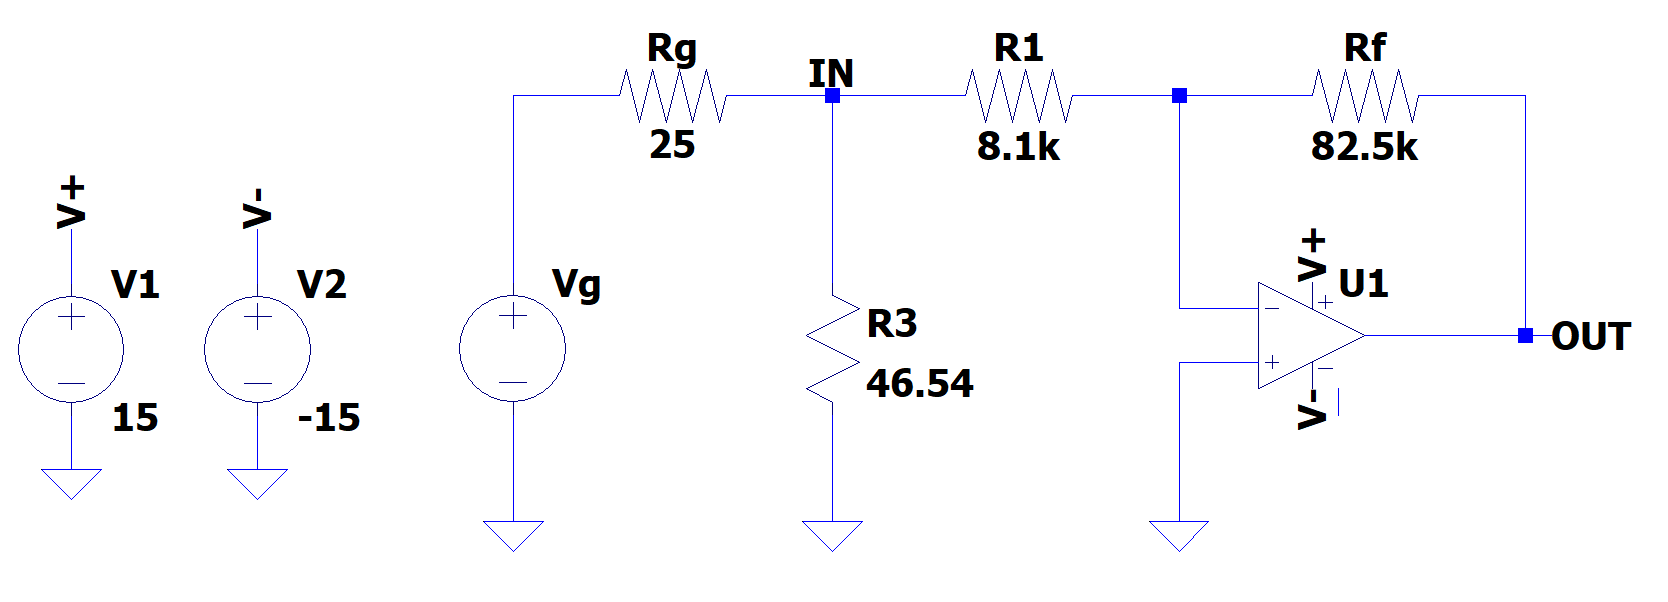
\includegraphics[width=0.6\textwidth]{../Simulations/OpAmp/circuit_image_nosim.png}
	\caption{\footnotesize Rappresentazione a variabili concentrate del circuito assemblato in laboratorio.}
	\label{i:opamp_circuit}
\end{wrapfigure}

\noindent direttamente utilizzando il multimetro Metrix MTX3292, ottenendo i risultati esposti in
\autoref{t:direct_measures}. Si utilizza poi un generatore di tensione continua con $V_{\text{cc}}=+15\,\si{\volt}$ e
$V_{\text{ee}}=-15\,\si{\volt}$ per l'alimentazione dell'amplificatore operazionale. Si assume, inoltre, che esso abbia
un comportamento ideale, ovvero che il polo positivo ed il polo negativo si trovino allo stesso potenziale. Il segnale
viene prelevato nei punti \textit{IN} e \textit{OUT} evidenziati nello schema in \autoref{i:opamp_circuit} (e verrà in
seguito richiamato rispettivamente come $V_{\text{in}}$ e $V_{\text{out}}$) utilizzando due sonde con fattore di
attenuazione 10X. Nel canale CH1 dell'oscilloscopio viene visualizzato il segnale in ingresso $V_{\text{in}}$, mentre il
segnale in uscita $V_{\text{out}}$ è prelevato dalla sonda collegata al canale CH2. Per entrambi i canali viene
selezionata la modalità "attenuazione sonda 10X", in modo da compensare la riduzione del segnale dovuta alle sonde e
visualizzare quindi nel display il segnale reale. Il generatore di funzioni viene poi configurato in

\begin{wraptable}{L}{0.5\textwidth}
	\small
	\centering
	\begin{tabular}{x{1.8cm} x{2.5cm} x{2cm} } \toprule[0.5px]\toprule[0.1px]
		
		\multicolumn{3}{c}{Misure Dirette delle Resistenze}\tn
		\midrule[0.1px]
		
		Resistenza & Valore & F.S. \tn
		
		\addlinespace
		
		$R_{\text{f}}$ & $82.46 \pm 0.03\,\si{k\ohm}$ & $100\,\si{k\ohm}$ \tn

		$R_1$ & $8.089 \pm 0.003\,\si{k\ohm}$ & $10\,\si{k\ohm}$ \tn

		$R_3$ & $46.54 \pm 0.05\,\si{\ohm}$ & $1\,\si{k\ohm}$ \tn
		
		\bottomrule[0.5px]		
	\end{tabular}
	\caption{\footnotesize Valori di resistenza, misurati direttamente con il multimetro, e relativo fondoscala.}
	\label{t:direct_measures}
\end{wraptable}	

\noindent  modalità "50 Ohm", in modo che l'impedenza d'uscita del generatore sia comparabile con
$R_3\approx 50\,\si{\ohm}$. Ci si aspetta così di trovare una tensione in ingresso $V_{\text{in}}$ in accordo con la
tensione nominale erogata dal generatore. Si imposta infine il generatore di funzioni in modo da erogare un segnale di
tipo sinusoidale con frequenza $f_{\text{gen}}=1\,\si{k\hertz}$, mantenuta costante in questa sezione, e di ampiezza
invece variabile tra $200\,\si{\mV}$ picco picco e $3.5\,\si{\V}$ picco picco. \\

\noindent Dall'assunzione di idealità dell'amplificatore operazionale segue che, risolvendo il circuito, il segnale in
uscita è legato a quello in ingresso da $V_{\text{out}} = - R_{\text{f}} / R_{1} \, V_{\text{in}}$, dove il segno meno
(dovuto alla particolare configurazione dell'operazionale) indica un segnale in output invertito\footnote{Ci si aspetta
che i massimi del segnale in ingresso corrispondano ai minimi del segnale in uscita e viceversa.} rispetto a quello in
ingresso, e amplificato di un fattore $G \equiv R_{\text{f}} / R_{1}$. Facendo riferimento ai valori
delle resistenze $R_{\text{f}}$ ed $R_1$ riportate in \autoref{t:direct_measures}, l'aspettativa teorica per il guadagno
del circuito è dunque 
\begin{align}\label{e:guadagno}
	G&=\frac{R_{\text{f}}}{R_{1}} = 10.194 \pm 0.006
	&
	\text{con   }\,\,\sigma_{G}&=\sqrt{	\left(	\frac{	1	}{	R_{1}	}	\right)^2	\sigma_{R_{\text{f}}}^2	
	+	\left(	\frac{	R_{\text{f}}	}{	R_{1}^2	}	\right)^2\sigma_{R_{1}}^2	}
\end{align}

%-------------------------------------------------------------------------------------------------------------------------------------------
%	SIMULAZIONE SPICE PRELIMINARE
%-------------------------------------------------------------------------------------------------------------------------------------------

\subsubsection{Simulazione Spice del Circuito}\label{s:spice} Si decide di effettuare una simulazione della risposta del
circuito ad un segnale sinusoidale di frequenza $f_{\text{gen}}=1\,\si{k\hertz}$ in ingresso, come da configurazione
sperimentale. In \autoref{i:opamp_simulation} sono rappresentate due 

\begin{wrapfigure}{L}{0.5\textwidth}
	\centering
	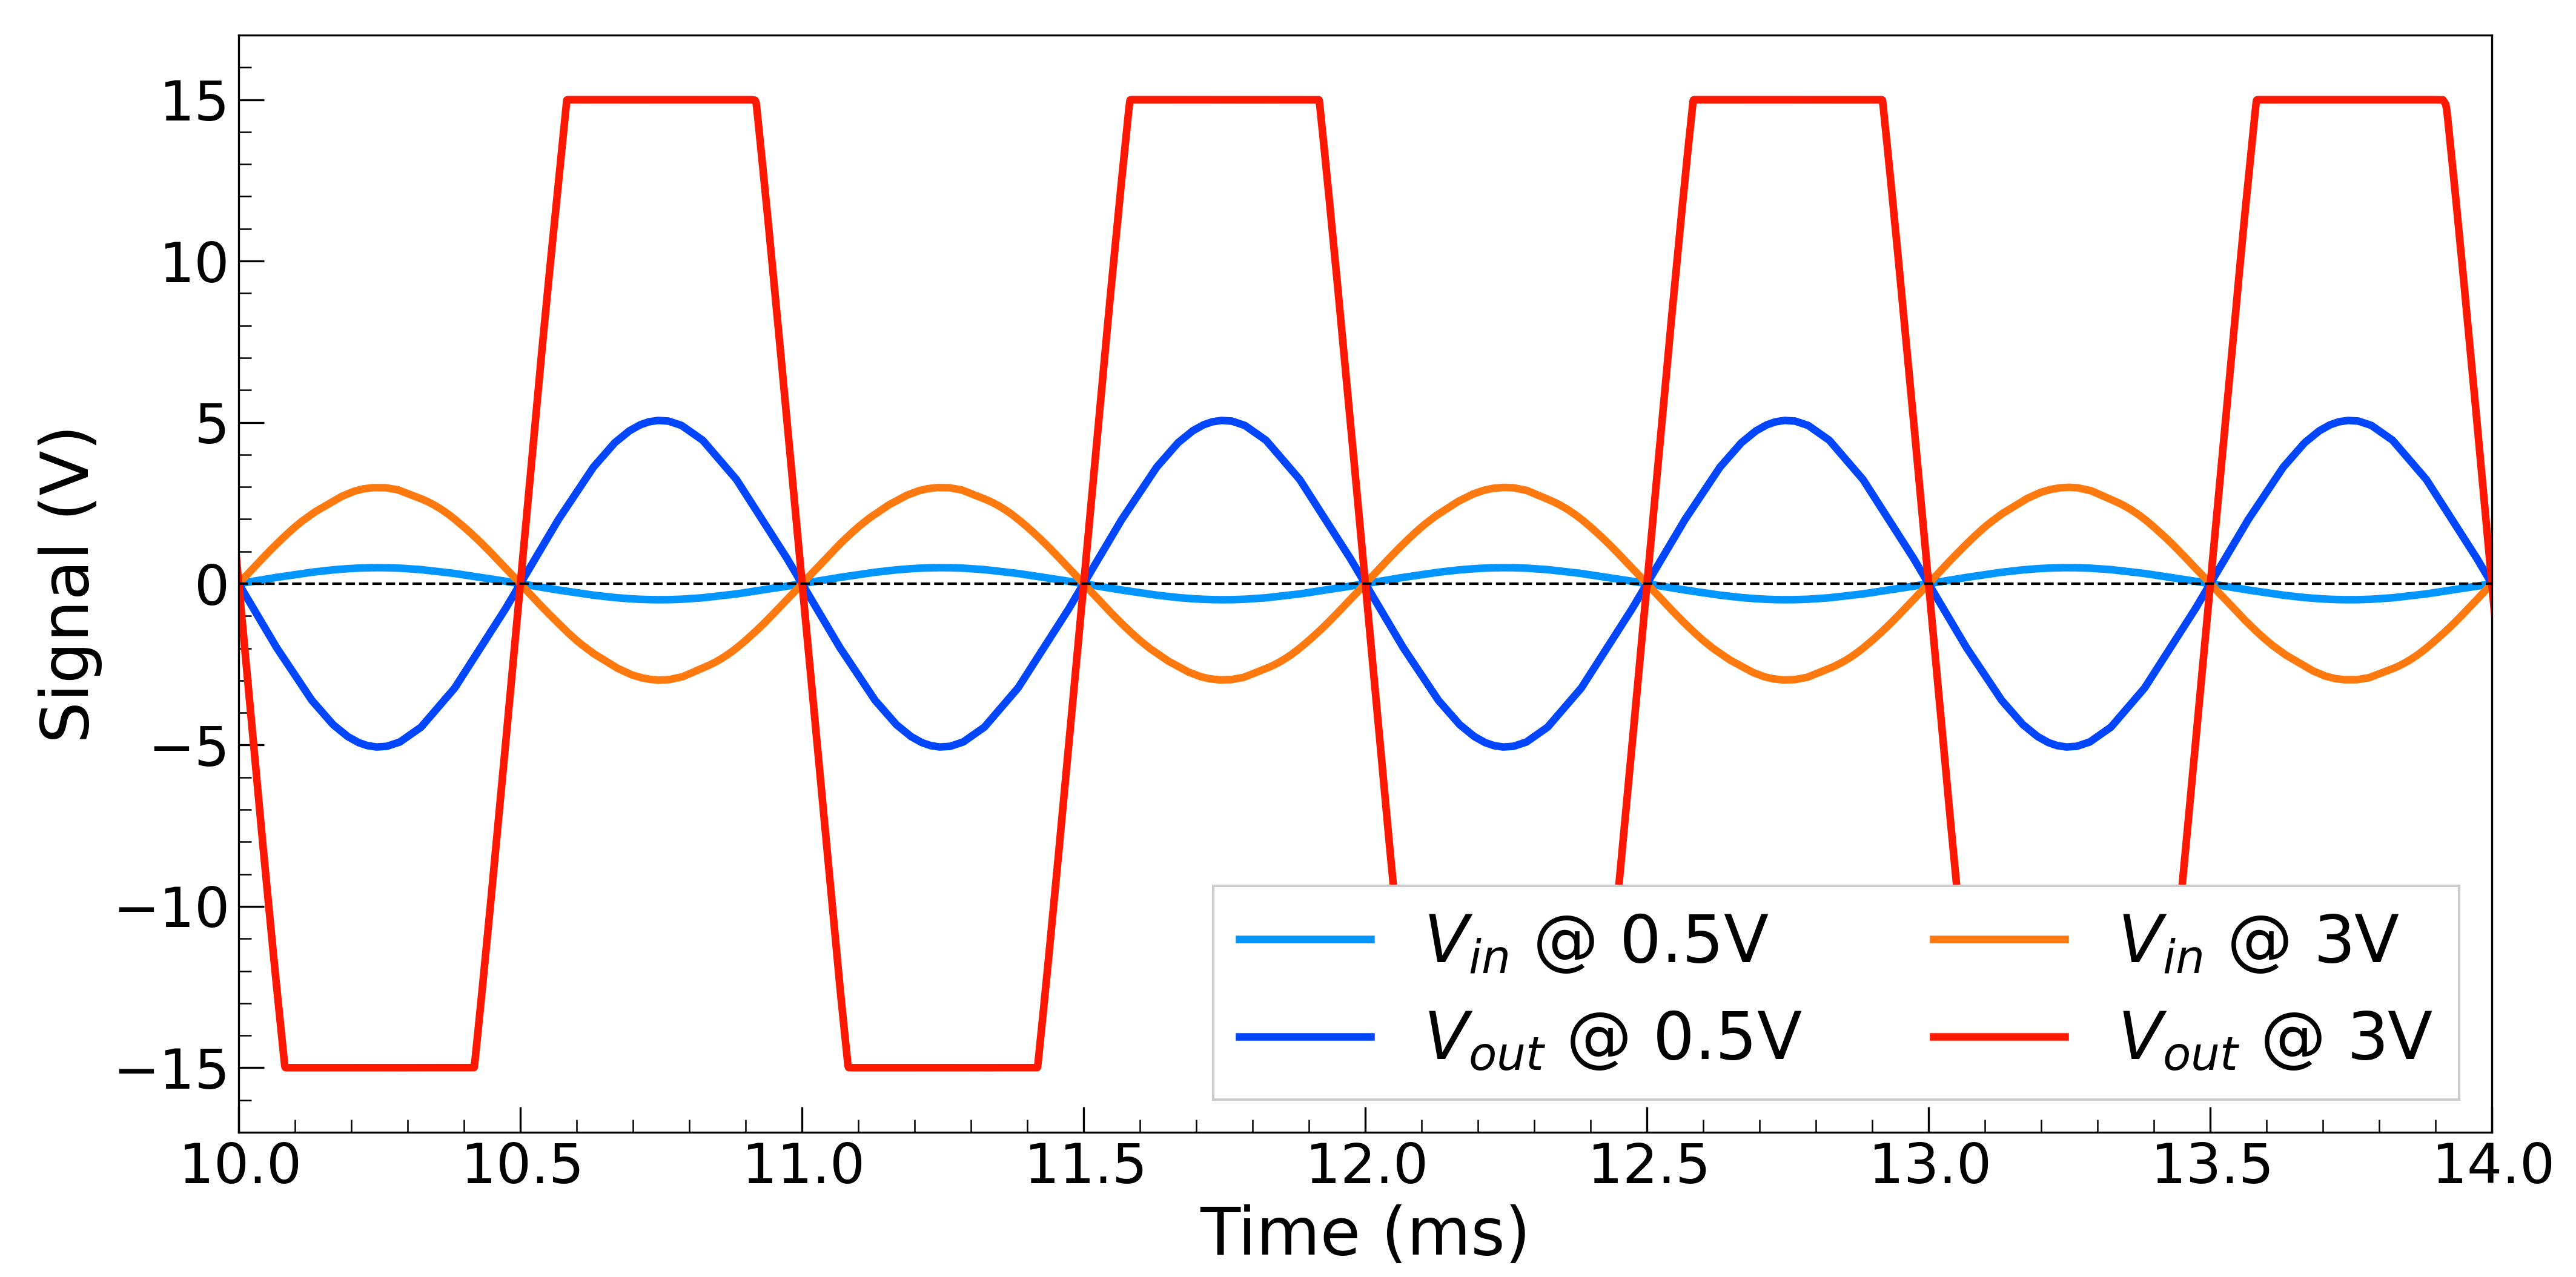
\includegraphics[width=0.5\textwidth]{../Plots/Report_Plots/opamp_spice_py.png}
	\caption{\footnotesize Simulazione Spice della risposta del circuito.}
	\label{i:opamp_simulation}
\end{wrapfigure}

\noindent simulazioni corrispondenti a due ampiezze differenti del segnale in ingresso: la prima (in tonalità
\textit{blu}) è la risposta a $V_{\text{gen}}=0.5\,\si{\volt}$, mentre la seconda (in tonalità \textit{rossa}) a
$V_{\text{gen}}=3\,\si{\volt}$. Dal grafico si nota chiaramente come la risposta $V_{\text{out}}$ ad un segnale in
ingresso $V_{\text{gen}}=0.5\,\si{\volt}$ sia perfettamente conforme alle aspettative: viene mantenuta la forma
sinusoidale del segnale, amplificato di circa un fattore 10 ed invertito rispetto alla tensione $V_{\text{in}}$. Si nota
inoltre come questo non si ripresenti anche nel caso della risposta a $V_{\text{gen}}=3\,\si{\volt}$: il segnale in
uscita presenta, infatti, i picchi di massimo e minimo tagliati a livello $V_{\text{sat}}=\pm 15\,\si{\volt}$. Questo
accade perchè, essendo l'amplificatore operazionale una componente attiva del circuito, è stato alimentato con una
tensione continua a $\pm 15\,\si{\volt}$ (come riportato sopra). Per la conservazione dell'energia, allora, l'operazionale
non può fornire in output una tensione maggiore di quanta ne riceve esso stesso in alimentazione. Si parla quindi di
\textit{saturazione} del segnale in uscita a $V_{\text{sat}}=\pm 15\,\si{\volt}$. Per quanto detto,  avendo $G \approx
10$, ci si aspetta che questo fenomeno inizi a manifestarsi attorno ad un valore nominale di tensione
$V_{\text{gen}}=1.5\,\si{\volt}$.


%-------------------------------------------------------------------------------------------------------------------------------------------
%	ACQUISIZIONE MISURE
%-------------------------------------------------------------------------------------------------------------------------------------------

\subsection{Acquisizione Misure}
Al fine di verificare la linearità dell'amplificatore operazionale e stimare l'amplificazione $G$ del circuito, vengono
acquisite separatamente le misure di un massimo ed un minimo sia del segnale in ingresso sia di quello in uscita facendo
variare la tensione nominale erogata dal generatore partedo da $200\,\si{\mV}$ picco picco fino a $3.5\,\si{\volt}$ picco
picco. Per l'acquisizione vengono utilizzati i cursori di tipo tensione (orizzontali) dell'oscilloscopio. 


%-------------------------------------------------------------------------------------------------------------------------------------------
%	DATI E ANALISI
%-------------------------------------------------------------------------------------------------------------------------------------------

\subsection{Dati e Analisi}
In questa sezione si vuole inizialmente rappresentare le misure acquisite in laboratorio riportandole in un grafico
esplorativo di $V_{\text{out}}$ contro $V_{\text{in}}$: da questo si cerca dunque di estrarre informazioni di carattere
generale riguardo i dati a disposizione. Le coppie $\{V_{\text{in}},\,V_{\text{out}}\}$ sono costruite associando, per
ogni valore di tensione nominale erogata dal generatore, il massimo di $V_{\text{out}}$ al rispettivo massimo di
$V_{\text{in}}$ (analogo per i minimi). Per quanto riportato in \autoref{s:guadagno} ci si aspetta una distribuzione
lineare delle coppie con pendenza pari all'amplificazione del circuito $G$: attraverso un'interpolazione lineare,
quindi, è possibile estrarre una stima di tale $G$. Inoltre è possibile caratterizzare la linearità dell'operazionale
tramite la bontà del fit e studiando l'andamento dei residui associati all'interpolazione.


%-------------------------------------------------------------------------------------------------------------------------------------------
%	DATISET
%-------------------------------------------------------------------------------------------------------------------------------------------

\subsubsection{Dataset}
Si comincia riportando in \autoref{i:opamp_eda} le misure acquisite con l'oscilloscopio. A queste, cioè sia a
$V_{\text{in}}$ che $V_{\text{out}}$, si associa l'incertezza
\begin{equation}\label{e:osc}
	\sigma_{V} = \sqrt{ (\sigma_{\text{L}}\times\text{V/div})^2 + (\sigma_{\text{k}}\times\text{measure})^2 }
\end{equation}
\noindent dove $\sigma_{\text{L}}=0.04$ rappresenta il contributo di lettura e $\sigma_{\text{k}}=1.5\%$ il contributo di scala
associati all'oscilloscopio mentre V/div rappresenta la scala di acquisizione della misura.

\begin{figure}[H]
	\centering
	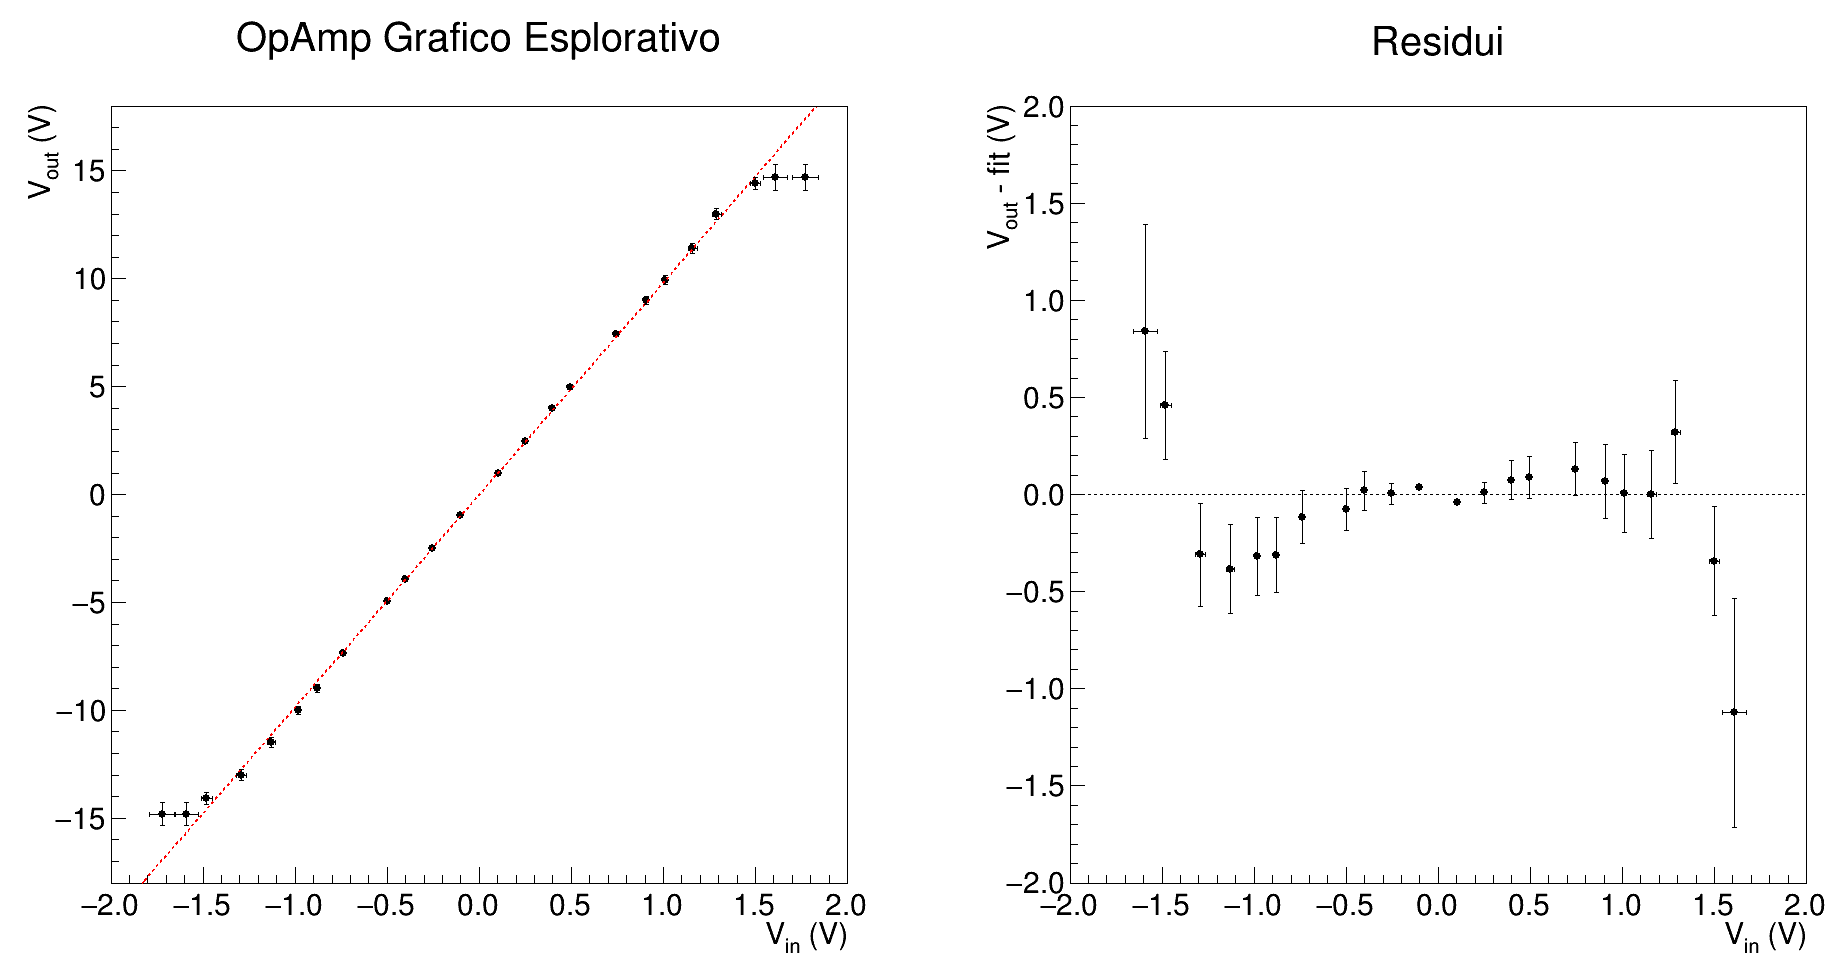
\includegraphics[width=\linewidth]{../Plots/Report_Plots/opamp_plot_alldata_eda.png}
	\caption{\small Grafico delle misure acquisite interpolate linearmente e relativo grafico dei residui.}
	\label{i:opamp_eda}
\end{figure}
\noindent Inizialmente, si vuole far notare che i valori di $V_{\text{in}}$ sono conformi a quanto erogato dal
generatore: questo è sicuramente indice di una corretta acquisizione del segnale in ingresso, di una corretta
configurazione del genetratore (modalità "50 Ohm") e dell'oscilloscopio (attenuazione sonda 10X). Osservando invece i
valori di $V_{\text{out}}$, si nota un'amplificazione conforme alle aspettative (circa un fattore 10). Si osserva,
inoltre, come le misure acquisite a $V_{\text{gen}}\approx 1.5\,\si{\volt}$ tendano a stabilizzarsi attorno a
$V_{\text{out}}=V_{\text{sat}}=\pm 15\,\si{\volt}$, ovvero la tensione massima che l'amplificatore operazionale può
fornire in output: questo effetto di saturazione del segnale in uscita è perfettamente conforme alle aspettative esposte
in \autoref{s:spice}. Spostando l'attenzione verso il grafico dei residui, si può notare chiaramente l'effetto della
saturazione del segnale: le misure acquisite in tale condizione risultano essere outliers rispetto al trend lineare dei
dati rimanenti (zona centra), i quali residui si distribuiscono ragionevolmente attorno allo zero. Quanto spazio ho
ancora?


%-------------------------------------------------------------------------------------------------------------------------------------------
%	PRELIMIARY FIT
%-------------------------------------------------------------------------------------------------------------------------------------------

\subsubsection{Interpolazioni Preliminari}\label{s:pre} Si procede ora considerando il campione di misure dei massimi ed
il campione di misure dei minimi separatamente, in quanto a priori non si ha la certezza che queste risentano della
stessa amplificazione e che non sia presente una sistematica di offset/shift verticale tra i due dataset. Si cercherà in
seguito di caratterizzare l'accordo tra i due dataset studiando la compatibilità tra i coefficienti angolari e tra le
intercette della retta interpolante. Osservando le misure in  \autoref{i:opamp_eda} si nota come le incertezze su
$V_{\text{in}}$ siano generalmente un ordine di grandezza inferiori rispetto a quelle su $V_{\text{out}}$: le prime non
sono quindi trascurabili rispetto alle seconde. Per tenere conto dell'incertezza su $V_{\text{in}}$, ci si propone
allora di effettuare un fit preliminare, nel quale si considerano unicamente gli errori su $V_{\text{out}}$, per stimare
un coefficiente angolare $m$. Questo viene poi utilizzato per proiettare gli errori di $V_{\text{in}}$ lungo l'asse
delle ordinate secondo 

\begin{equation}\label{e:proj}
	\sigma_{y} = \sqrt{	\sigma_{V_{\text{out}}}^2	+	m^2	\sigma_{V_{\text{in}}}^2	}
\end{equation}

\noindent I coefficienti angolari di interesse sono dunque riportati in  \autoref{t:pre_slopes}.

\begin{table}[H]
	\small
	\centering
	\begin{tabular}{x{4cm} x{4cm}} 

		\toprule[0.5px]
		\toprule[0.1px]
		
		\multicolumn{2}{c}{Coefficienti Angolari Preliminari}\tn
		\midrule[0.1px]

		Campione di Massimi & Campione di Minimi \tn

		\addlinespace
		
		$m=10.02\pm0.09$ & $m=10.16\pm0.09$ \tn
		
		\bottomrule[0.5px]
		
	\end{tabular}
	\caption{\small Valori dei coefficienti angolari restituiti dalle interpolazioni preliminari.}
	\label{t:pre_slopes}
\end{table}	

%-------------------------------------------------------------------------------------------------------------------------------------------
%	LINEARITA E AMPLIFICAZIONE
%-------------------------------------------------------------------------------------------------------------------------------------------


\subsubsection{Linearità e Amplificazione}
Alla luce di quanto trovato nella sezione precedente, si ripetono le interpolazioni lineari associando ai punti un
errore dato da  \autoref{e:proj} ed i parametri restituiti dai fit sono riportati in  \autoref{t:opamp_fitres_max_min}.

\begin{table}[H]
	\centering
	\small
	\begin{tabular}{x{3cm} x{3cm} x{3cm} x{3cm}} 

		\toprule[0.5px]
		\toprule[0.1px]
		
		\multicolumn{4}{c}{Fit Parameters}\tn
		\midrule[0.1px]

		\multicolumn{4}{c}{Campione di Massimi}\tn

		\addlinespace
		
		Offset (V) & Slope & $\chi^2$/ndf & $\sigma_{\text{posteriori}}$ (V)\tn

		\addlinespace

		$-0.06\pm0.04$ & $10.02\pm0.14$ & $0.98/7$ & $0.10$ \tn

		\midrule[0.1px]
		
		\multicolumn{4}{c}{Campione di Minimi}\tn

		\addlinespace
		
		Offset (V) & Slope & $\chi^2$/ndf & $\sigma_{\text{posteriori}}$ (V) \tn

		$0.07\pm0.04$ & $10.16\pm0.14$ & $0.67/7$ & $0.07$ \tn



		\bottomrule[0.5px]
		
	\end{tabular}
	\caption{\small Parametri della retta interpolante, il valore del $\chi^2$ associato al fit 
	e l'errore a posteriori relativo alla distribuzione dei dati.}
	\label{t:opamp_fitres_max_min}
\end{table}	

\noindent Dai parametri presentati in  \autoref{t:opamp_fitres_max_min} si riescono ad estrarre numerose informazioni
riguardo ai due campioni di dati. Inizialmente, si vuole far notare come i due coefficienti angolari siano in ottima
compatibilità tra loro: $\lambda=0.7$. Da questo si può assumere che i due dataset risentano della stessa amplificazione
$G$, come da aspettative. Successivamente, si può notare invece che le due intercette delle rette interpolanti sono in
leggera compatibilità con lo zero ($\lambda \approx 1.5$), mentre tra loro presentano una compatibilità $\lambda=2.4$,
che fa sorgere l'idea di una possibile sistematica di offset/shift verticale tra i due dataset (computando la differenza tra le
due intercette si trova uno sfalsamento $d=0.13 \pm 0.05 \,\si{\volt}$). Osservando poi il valore del $\chi^2$, si
ritrova in per entrambi i campioni $\chi^2/\nu<1$ (con $\nu\equiv\text{ndf}$ il numero di gradi di libertà, che coincide
con il valore di aspettazione $E(\chi^2)$). Ricordando che le incertezze sul guadagno verticale dell'oscilloscopio sono
almeno parzialmente correlate, gli errori associati alle misure sono tra loro correlati: questo spiega i valori di
$\chi^2$ eccessivamente ridotti. Un'interpolazione di dati con incertezze correlate restituisce parametri con errori
sottostimati, in quanto il fit non tiene conto della correlazione tra incertezze delle misure. Si può dunque assumere
che i parametri \textit{slope} e \textit{offset} riportati in \autoref{t:opamp_fitres_max_min} presentino in realtà una
compatibilità maggiore, proprio a causa di una possibile sottostima dell'errore sui parametri. Si vuole allora assumere
che i due campioni risentano della stessa amplificazione e che non siano tra loro sfalsati verticalmente in modo
significativo: segue quindi un tentativo di "unificazione" del campione di dati ed un'interpolazione lineare unica che
tenga conto sia dei massimi che dei minimi. Il grafico rappresentante i due dataset unificati con relativa
interpolazione lineare è mostrato in \autoref{i:opamp_all_proj}. 
%-------------------------------------------------------------------------------------------------------------------------------------------
%	FIT UNIFICATO
%-------------------------------------------------------------------------------------------------------------------------------------------
\begin{figure}[H]
	\centering
	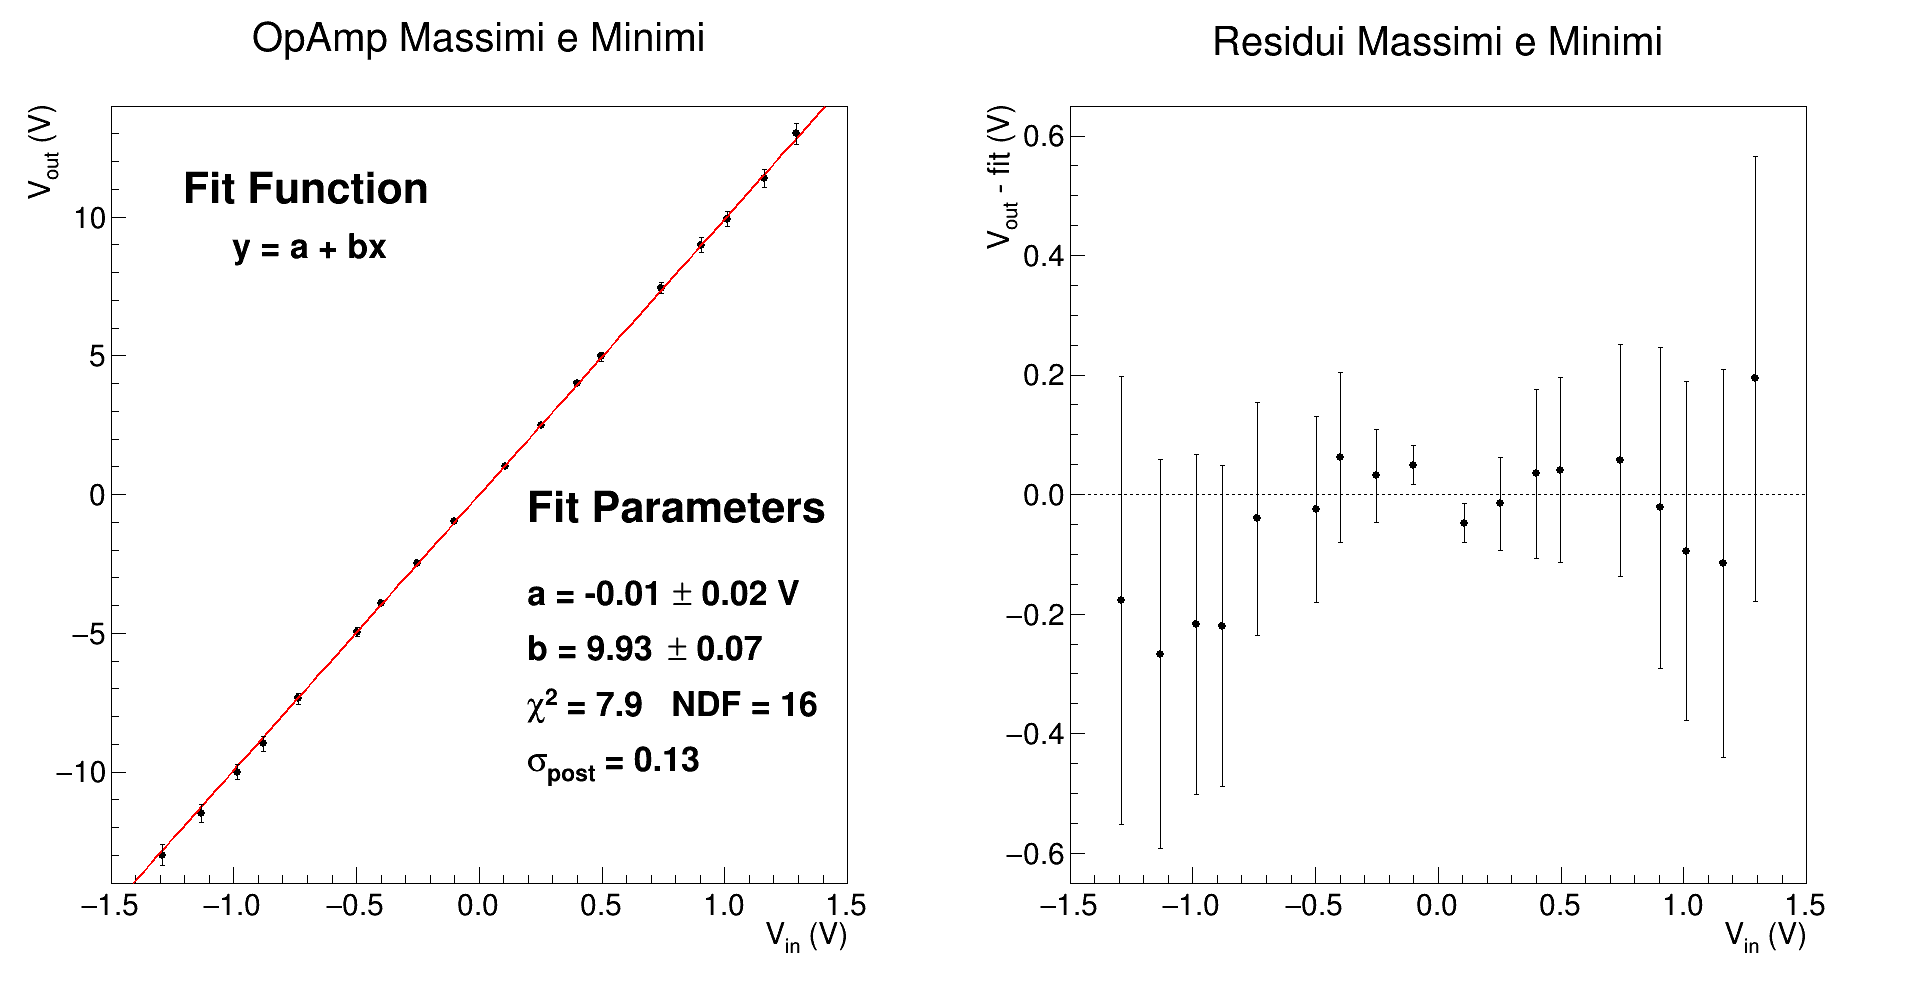
\includegraphics[width=\linewidth]{../Plots/Report_Plots/opamp_plot_all_projected.png}
	\caption{\small A sinistra: grafico rappresentante il dataset dei massimi ed il dataset dei minimi uniti assieme, 
	con relativa retta interpolante e parametri del fit. A destra: grafico dei residui $V_{\text{out}}-\text{fit}$.}
	\label{i:opamp_all_proj}
\end{figure}

\noindent Si osserva inizialmente che l'intercetta della retta interpolante è ora ben compatibile con zero, mentre il
coefficiente angolare presenta un errore relativo $\sigma_{b}/b=0.7\%$, che si può continuare ad assumere sottostimato:
la correlazione tra gli errori di scala, infatti, si può notare chiaramente dall'andamento "a farfalla" delle barre
d'errore nel grafico dei residui. Il valore del $\chi^2$ migliora leggermente rispetto alle interpolazioni dei dataset
separati: la compatibilità con il valore di aspettazione risulta essere $Z=1.4$. L'errore a posteriori, inoltre, si
trova in una zona intermedia rispetto alla gamma di errori associati alle misure: non potendo eliminare la correlazione
tra le incertezze si può affermare dunque che l'errore è in media stimato correttamente e l'oscilloscopio lavora entro
le specifiche. I residui, infatti, si posizionano tutti entro il loro errore, alcuni anche abbondantemente.
Focalizzandosi ora sulla stima del coefficiente angolare si nota che questo, $m=9.93\pm 0.07$, pur essendo ben
compatibile con i risultati esposti in  \autoref{t:opamp_fitres_max_min} relativi ai fit dei due campioni di misure
considerati separatamente, si trova essere sensibilmente minore di entrambi: ci si sarebbe aspettato, invece, di trovare
un valore intermedio unificando i due campioni di misure. Osservando poi il grafico dei residui, si può notare un
andamento leggermente anomalo, quasi parabolico, avente concavità rivolta verso il basso. Si ipotizza dunque che
l'assunzione fatta in precedenza riguardo la presenza di una sistematica di offset/shift verticale tra i due dataset
trascurabile necessiti di essere rivisitata. Per approfondire maggiormenta la questione, si decide di computare le
grandezze "picco picco" delle tensioni in ingresso $V_{\text{in}}$ e in uscita $V_{\text{out}}$ secondo
$V_{\text{pp}}=V^{\text{max}}-V^{\text{min}}$. Per quanto riguarda l'errore da associare alle grandezze picco picco, si
ricorda che l'oscilloscopio misura la differenza $\Delta$ tra i due cursori con una precisione ancora maggiore rispetto
alla singola misura. Si decide dunque di non aggiungere il fattore moltiplicativo $\sqrt{2}$ alla propagazione
presentata in  \autoref{e:osc}, al fine di evitare sovrastime eccessive dell'errore. Si procede ora come mostrato in
\autoref{s:pre}, effettuando inizialmente un fit lineare preliminare considerando solo gli errori su $Vpp_{\text{out}}$
e, utilizzando il coefficiente angolare restituito da tale interpolazione, si prosegue proiettando gli errori secondo
\autoref{e:proj}. Si ripete quindi il fit, che viene rappresentato in \autoref{i:opamp_pp}. Osservando il grafico dei
residui, si nota immediatamente come ora l'andamento anomalo è del tutto assente ed i punti si distribuiscono in modo
ottimale attorno allo zero. Rimane, chiaramente, il tipico andamento crescente delle barre d'errore, indice che le
incertezze continuano a risentire della correlazione tra esse. Il valore del $\chi^2$ è decisamente basso rispetto al
numero di gradi di libertà, come suggerito dal grafico dei residui in cui si nota chiaramente come la distanza
punto-retta sia ampiamente compresa entro la barra d'errore del dato. L'errore a posteriori è appena maggiore
dell'incertezza associata al primo punto, mentre diventa notevolmente inferiore per i successivi.
%-------------------------------------------------------------------------------------------------------------------------------------------
%	FIT PICCO PICCO
%-------------------------------------------------------------------------------------------------------------------------------------------
\begin{figure}[H]
	\centering
	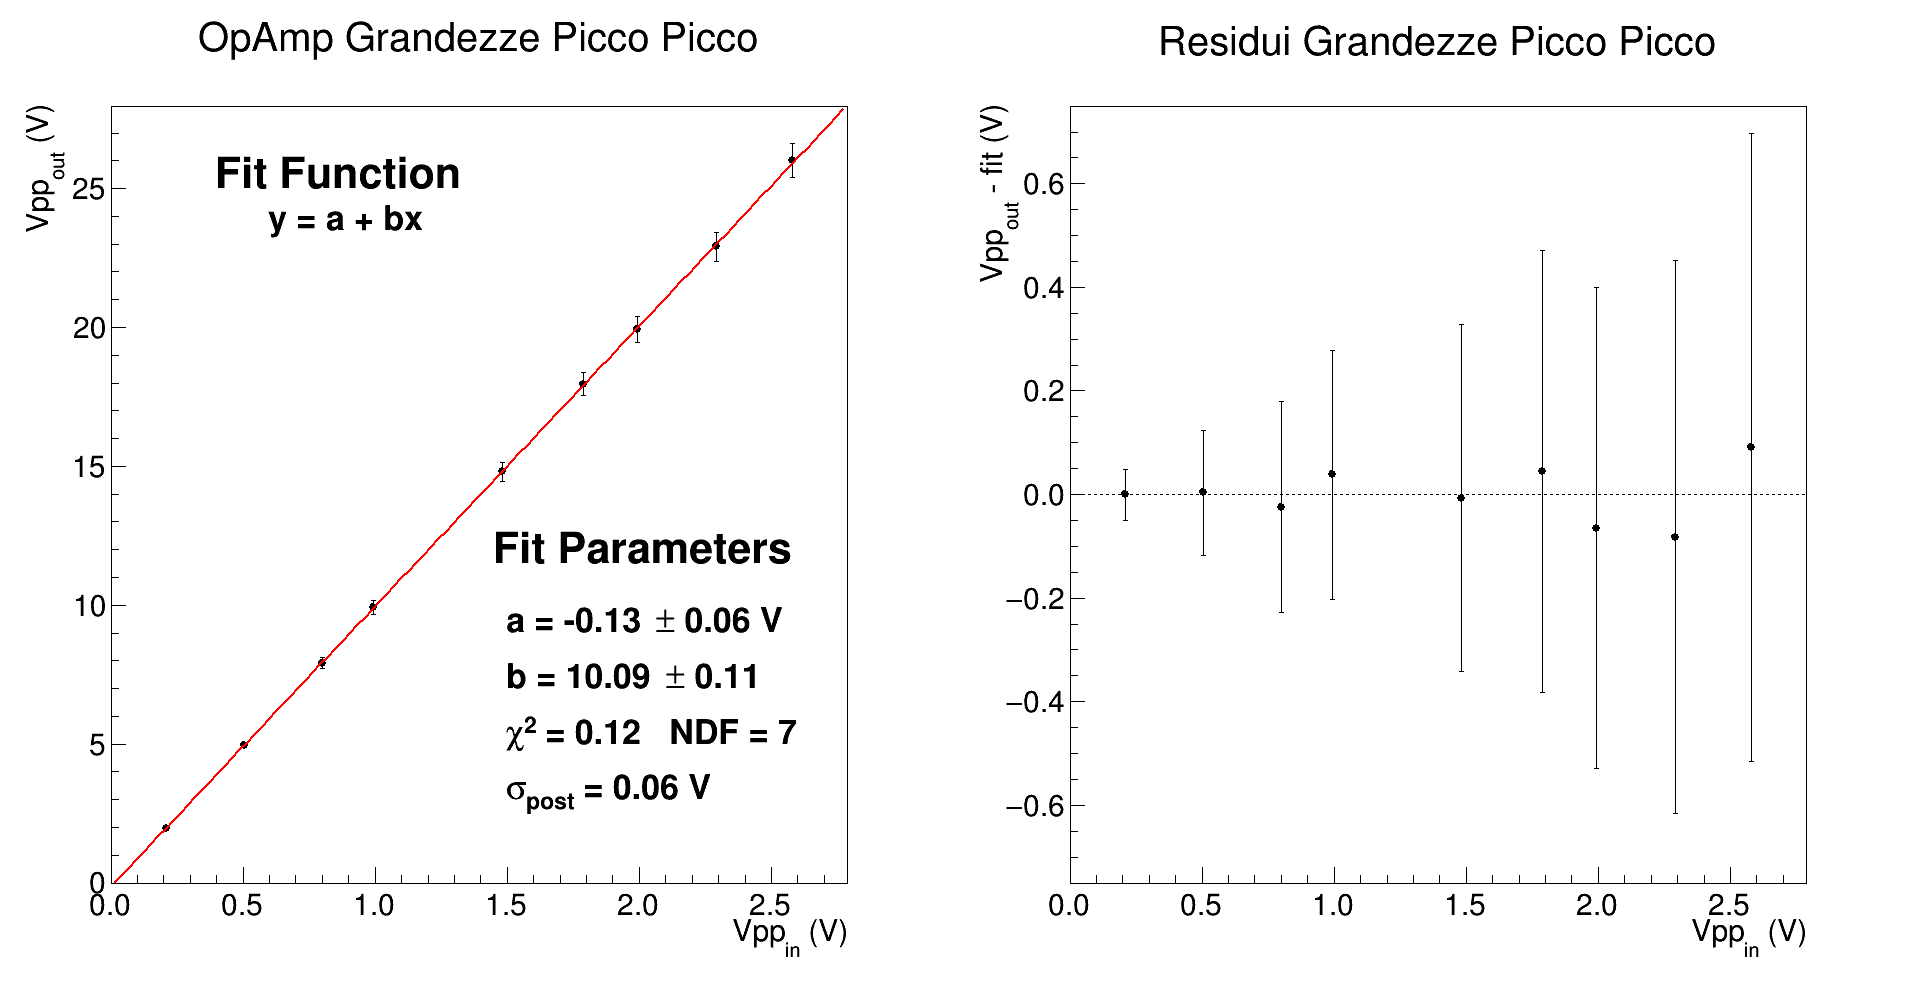
\includegraphics[width=\linewidth]{../Plots/Report_Plots/opamp_plot_pp_projected.png}
	\caption{\small A sinistra: grafico rappresentante il dataset delle grandezze picco picco, 
	con relativa retta interpolante e parametri del fit. A destra: grafico dei residui $V\text{pp}_{\text{out}}-\text{fit}$.}
	\label{i:opamp_pp}
\end{figure}

\noindent  Il valore dell'intercetta, scarsamente compatibile con lo zero, suggerisce una conferma all'ipotesi un una
sistematica di offset/shift verticale tra i due dataset non trascurabile. Il coefficiente angolare, invece, è
perfettamente in linea con i parametri ottenuti considerando i due dataset separatamente: calcolando la media pesata dei
due, infatti, si trova $\langle m\rangle_{\text{max, min}}=10.09 \pm 0.10$ e risulta avere una compatibilità
estremamente elevata con il coefficiente angolare riguardante il dataset delle grandezze picco picco ($\lambda = 0.01$).
Si assume dunque che questi due valori ($\langle m\rangle_{\text{max, min}}$ ed il coefficiente angolare del campione di
grandezze picco picco $m_{\text{pp}}$) rappresentino una soddisfacente stima dell'amplificazione \textit{G} del
circuito. Per quanto riguarda la linearità dell'amplificatore operazionale, invece, i valori estremamente ridotti del
$\chi^2$ non permettono nè di confermare l'ipotesi di linearità nè di poterla rigettare. Si ripone allora maggior
attenzione alla distribuzione delle misure attorno alla retta (o meglio alla distribuzione dei residui attorno allo
zero) che si ritiene invece, in questa occasione, determinante: il campione di misure picco picco suggerisce una
soddisfacente distribuzione lineare dei dati. 


%-------------------------------------------------------------------------------------------------------------------------------------------
%	CONFRONTO STIME DI G
%-------------------------------------------------------------------------------------------------------------------------------------------

\subsubsection{Confronto tra Stime di G}
 Si vuole ora esporre e confrontare le stime dell'amplificazione del circuito, rappresentando i valori del guadagno
\textit{G} in \autoref{i:opamp_comp}. Partendo dal primo punto a sinistra, cioè la stima di \textit{G} tramite le misure
dirette delle resistenze $R_{\text{f}}$ e $R_{1}$ (riportate in \autoref{t:direct_measures}), si nota come questo
presenti un errore 

\begin{wrapfigure}{L}{0.5\textwidth}
	\centering
	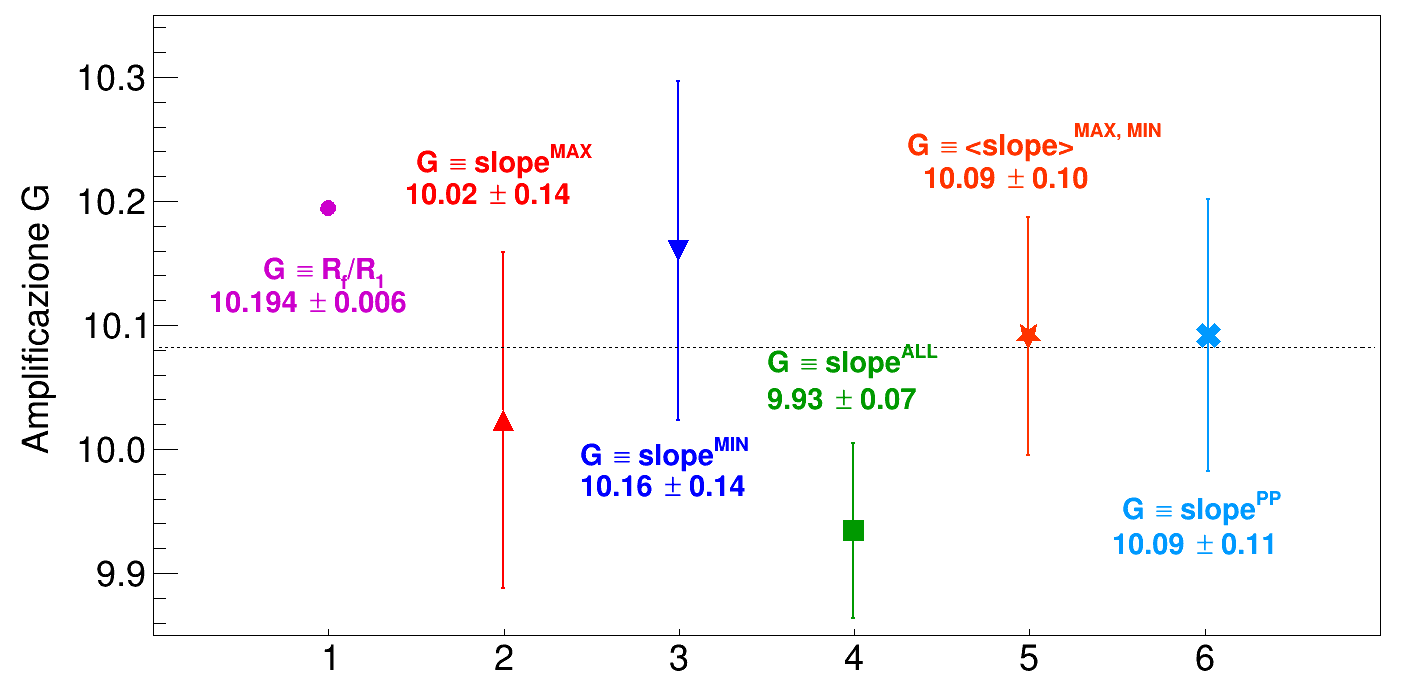
\includegraphics[width=0.5\textwidth]{../Plots/Report_Plots/opamp_comp_BIG.png}
	\caption{\footnotesize Stime di G. Da sinistra: 1) partendo dalle misure dirette delle resistenze; 2) come
	coefficiente angolare del dataset di massimi; 3) come coefficiente angolare del dataset di minimi; 4) come
	coefficiente angolare del dataset unificato; 5) come media pesata di 2 e 3; 6) come coefficiente angolare del
	dataset delle grandezze picco picco.}
	\label{i:opamp_comp}
\end{wrapfigure}

\noindent nettamente inferiore a confronto con le rimanenti stime. Quest'ultime risultano essere quantità compatibili
con 1) $G=R_{\text{f}}/R_{1}$, ad eccezione di 4) quella ottenuta considerando assieme sia i massimi sia i minimi
($\lambda = 3.7$). In particolare, si può osservare come la media pesata 5) tra le stime dell'amplificazione ottenute
considerando i campioni separati e la stima ottenuta con le grandezze picco picco 6) si trovino in eccellente accordo:
si può concludere dunque che, eliminando la sistematica di offset/shift verticale tra i due dataset (sia attraverso
grandezze picco picco, sia considerando la media pesata dei risultati ottenuti dai campioni separati), la stima
dell'amplificazione del circuito risulta essere compatibile con le aspettative preliminari. Si assume in ogni caso che
l'errore su \textit{G} sia sottostimato a causa della correlazione delle incertezze: si preferisce dunque la stima
ritrovata considerando le tensioni picco picco 6), in quanto presenta un errore relativo leggermente maggiore.


%-------------------------------------------------------------------------------------------------------------------------------------------
%	CIRCUITO DERIVATORE
%-------------------------------------------------------------------------------------------------------------------------------------------

\section{Filtro Attivo - Circuito Derivatore}
Ci si propone di studiare il comportamento \textit{in frequenza} di un circuito simile a quello
considerato in \autoref{s:opamp}, con l'aggiunta di un condensatore $C_{1}$ in serie alla resistenza $R_{1}$: questo lo
rende dunque un filtro (attivo, in quanto è sempre presente l'amplificatore operazionale) passa alto, derivatore a basse
frequenze. 

%-------------------------------------------------------------------------------------------------------------------------------------------
%	CONFIGURAZIONE SPERIMENTALE
%-------------------------------------------------------------------------------------------------------------------------------------------

\subsection{Configurazione Sperimentale}
Utilizzando la stessa configurazione circuitale rappresentata in \autoref{i:opamp_circuit}, viene aggiunta la capacità
$C_{1} = 0.977 \pm 0.017 \,\si{n\farad}$ (misurata direttamente utilizzando il multimetro digitale a fondo scala
$1\,\si{n\farad}$) in serie alla resistenza $R_{1}$, tra essa e l'amplificatore operazionale. Nel dominio delle
frequenze la funzione di trasferimento $H(s)=V_{\text{out}}(s)/V_{\text{in}}(s)$ del circuito risulta essere 
\begin{align}
	H(s) &= -\frac{R_{\text{f}}}{R_{1}}\frac{s}{s+\omega_{0}} & \text{con}\,\,\,\, \omega_{0}&=\frac{1}{R_{1}C_{1}}
\end{align}

\noindent Si nota dunque che il termine $-\frac{R_{\text{f}}}{R_{1}}$ è esattamente il guadagno $G$ (il segno meno è
sempre legato al fatto che l'operazionale è posto in configurazione invertente) del circuito studiato in
\autoref{s:opamp}, mentre il termine $\frac{s}{s+\omega_{0}}$ risulta essere analogo alla funzione di trasferimento di
un circuito passa alto passivo. Ci si aspetta dunque che a basse frequenze il circuito si comporti come un derivatore,
mentre, essendo un passa alto, ci si aspetta si ottenga il massimo guadagno per $s\rightarrow\infty$ e che questo sia
esattamente $G$. Si imposta allora il generatore in modo da erogare un'onda sinusoidale di ampiezza $1\,\si{\volt}$
picco picco (che verrà mantenuta costante) e frequenza variabile tra $100\,\si{\Hz}$ e $1\,\si{\MHz}$ per lo studio
della risposta in frequenza del circuito. Avendo misurato le componenti circuitali direttamente con i multimetri, la
stima attesa del massimo guadagno è già stata esplicitata in \autoref{e:guadagno}, mentre ci si aspetta una frequenza di
taglio

\begin{align}\label{e:diff_f_th}
	f_{\text{t}}&=\frac{1}{2\pi R_{1}C_{1}}=20.1 \,\si{k\Hz} & \sigma_{f_{\text{t}}}&=\frac{1}{2\pi}\sqrt{	\left(\frac{1}{C_{1}R_{1}^2}\right)^2\sigma_{R_{1}}^2	+
																	\left(\frac{1}{C_{1}^2R_{1}}\right)^2\sigma_{C_{1}}^2   }
																	= 0.3 \,\si{k\Hz}	
\end{align}


%-------------------------------------------------------------------------------------------------------------------------------------------
%	ACQUISIZIONE MISURE
%-------------------------------------------------------------------------------------------------------------------------------------------

\subsection{Acquisizione Misure}
Per studiare la risposta in frequenza del circuito, si fa variare la frequenza del segnale in ingresso da
$100\,\si{\Hz}$ a $1\,\si{\MHz}$ e vengono acquisite misure di tensione picco picco sia del segnale in ingresso sia di
quello in uscita: inizialmente viene effettuata un'acquisizione preliminare con il fine di individuare gli intervalli di
frequenze più interessanti, quali l'intorno della frequenza di taglio e l'intorno del massimo di amplificazione (si
trova infatti che questo non viene assunto al tendere della frequenza verso valori sempre maggiori, ma piuttosto si ha
un fenomeno di attenuamento di amplificazione oltre un certo range di frequenze). Così facendo, si riesce a fornire una
stima approssimativa della frequenza di taglio. Infatti, infittendo le misure in tali intervalli si trova
l'amplificazione massima sperimentale ($G_{\text{sper}}\approx 9.8$): questa viene divisa per un fattore $\sqrt{2}$ e,
successivamente, si ricerca la frequenza che corrisponde a tale amplificazione ridotta, sempre infittendo le misure
nell'intorno della frequenza di taglio. Si trova quindi $f_{\text{t, sper}}\approx 19.5\,\si{k\Hz}$, leggermente minore
rispetto a quanto trovato in \autoref{e:diff_f_th}.


%-------------------------------------------------------------------------------------------------------------------------------------------
%	DATI E ANALISI
%-------------------------------------------------------------------------------------------------------------------------------------------

\subsection{Dati e Analisi}
In questa sezione si vuole studiare il grafico di Bode relativo alle misure acquisite sperimentalmente sia con il fine di estrarre
informazioni di carattere generale sui dati, sia per fornire una stima della frequenza di taglio attraverso
l'interpolazione delle misure.


%-------------------------------------------------------------------------------------------------------------------------------------------
%	THEBODE
%-------------------------------------------------------------------------------------------------------------------------------------------

\subsubsection{Grafico di Bode}
Date le misure di tensione $V_{\text{in}}$ e $V_{\text{out}}$, viene calcolata la funzione di trasferimento
\begin{align}\label{e:diff_err}
	H&=\frac{V_{\text{out}}}{V_{\text{in}}} & \sigma_{H}&= H \sqrt{	
											\left(	\frac{	\sigma_{\text{L}}\times V_{\text{in}}/\text{div}	}{	V_{\text{in}}	}	\right)^2	 + 
											\left(	\frac{	\sigma_{\text{L}}\times V_{\text{out}}/\text{div}	}{	V_{\text{out}}	}	\right)^2 +	
											2\left(	\frac{	\sigma_{\text{k}}	}{	k	}	\right)^2 }	
\end{align}
\noindent dove $\sigma_{\text{L}}=0.04$ rappresenta l'incertezza di lettura associata all'oscilloscopio, i termini
$V_{\text{in}}/\text{div}$ e $V_{\text{out}}/\text{div}$ corrispondono al numero di volt per divisione per il canale di
acquisizione rispettivamente del segnale in ingresso e del segnale in uscita, mentre $\sigma_{\text{k}}=1.5\%$ rappresenta
l'incertezza di guadagno associata all'oscilloscopio: quest'ultima viene considerata in quanto le misure non sono state
acquisite utilizzando un'unica scala e, inoltre, sono state acquisite utilizzando due diversi canali. Si assume che $k$
sia mediamente pari all'unità. L'incertezza sulla frequenza dell'onda erogata dal generatore si assume trascurabile. Si
rappresenta allora in \autoref{i:diff_bode} il grafico di Bode delle misure acquisite assieme ai punti simulati con
LTSpice. Osservando il grafico si nota che sono state effettuate due interpolazioni: la prima lineare, per la quale sono
state considerate le prime tre misure, mentre la seconda parabolica, per la quale sono state considerate le misure
nell'intorno del massimo di amplificazione. La strategia per stimare la frequenza di taglio è la seguente: si stima il
massimo della funzione di trasferimento come vertice della parabola, si considera quindi la retta orizzontale
$y=H_{\text{max}}$ e si calcola il punto di intersezione con la retta $y=a+bx$ interpolante le prime tre misure
crescenti. In questo modo, la coordinata $x$ del punto di intersezione coincide con la frequenza di taglio del circuito.
Prima di discutere la frequenza di taglio del circuito, tuttavia, si vogliono fare delle considerazioni di carattere più
generale sul campione di dati rappresentato in \autoref{i:diff_bode}. Per la parte lineare (a sinistra) si può notare un
soddisfacente accordo tra misure sperimentali e dati simulati, e lo stesso vale nell'intorno della frequenza di taglio e
nell'intorno del massimo della funzione di trasferimento. Per questo motivo si può affermare che, siccome nell'analisi
per la ricerca della frequenza di taglio vengono utilizzate le misure che sono in accordo con le aspettative, i
risultati sono da considerarsi significativi.  

\begin{figure}[H]
	\centering
	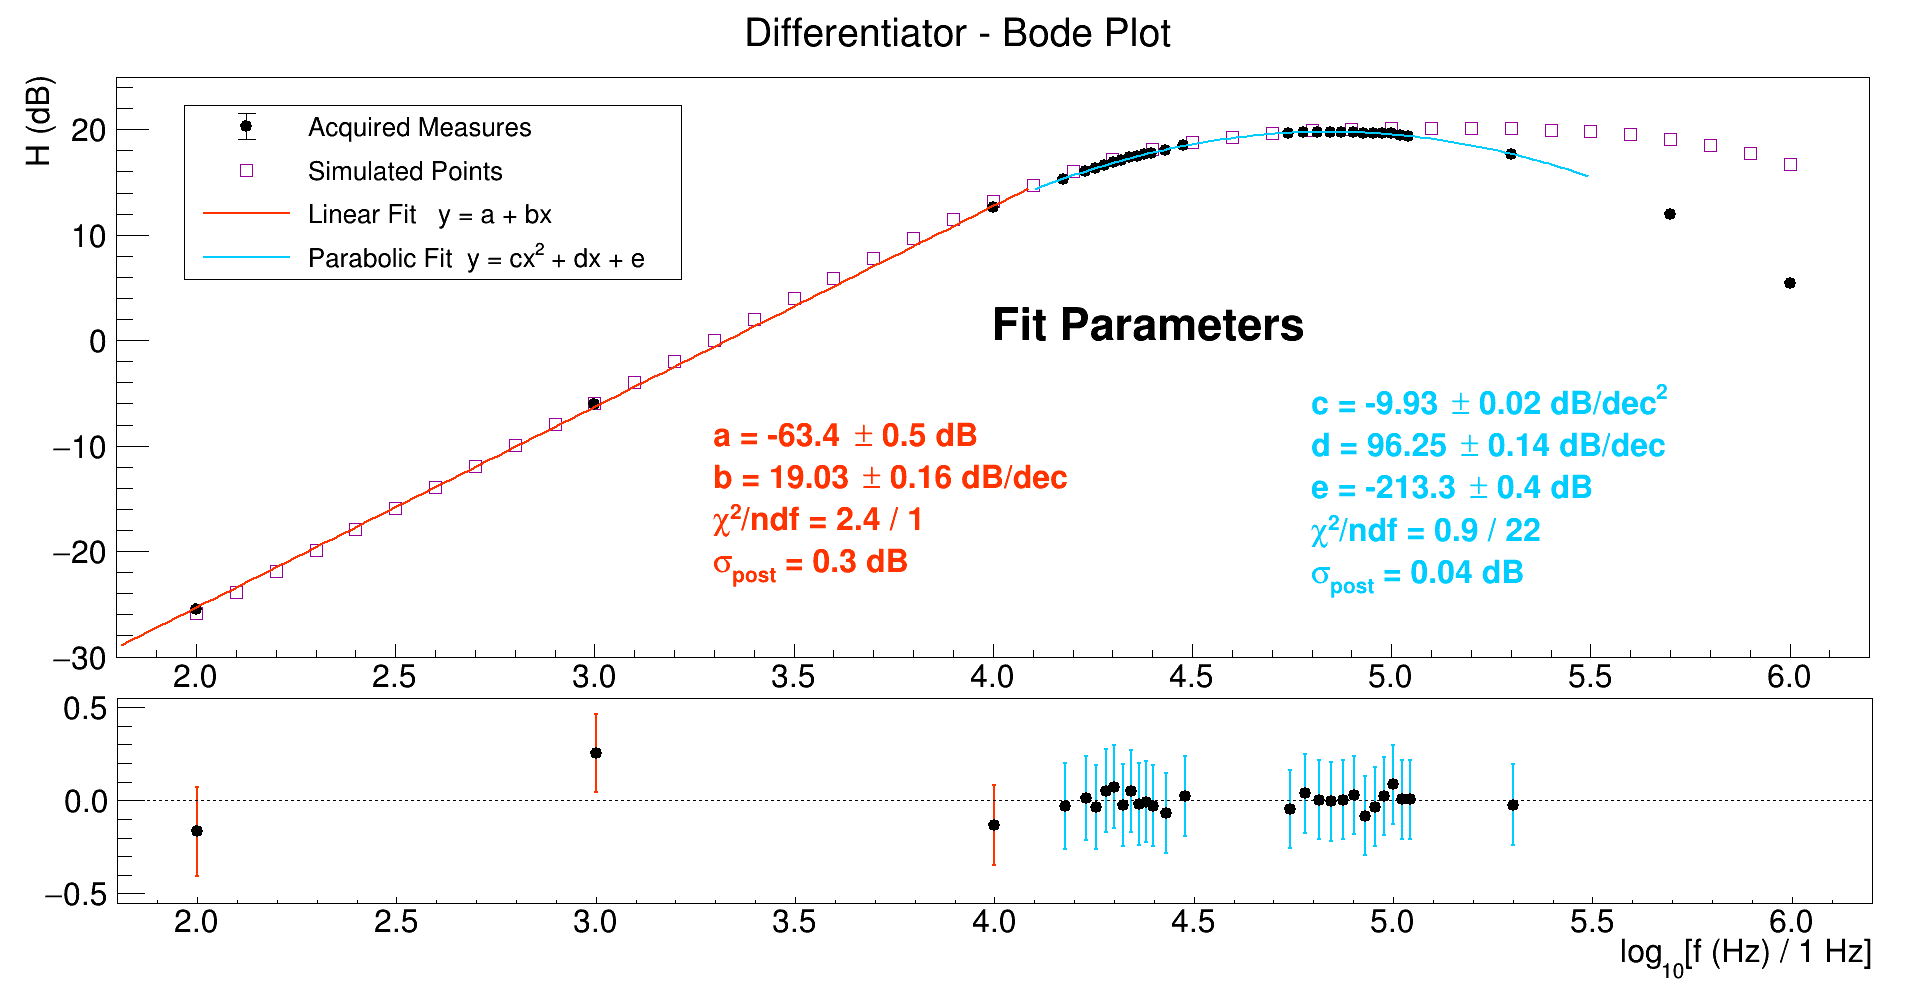
\includegraphics[width=\linewidth]{../Plots/Report_Plots/diff_bode.png}
	\caption{\small Grafico di Bode delle misure sperimentali e dei dati simulati. Le misure sperimentali vengono
	interpolate con una retta $y = a + bx$ e con una parabola $y = cx^2+dx+e$. Vengono mostrati anche i residui, 
	rispettivamente per la retta e per la parabola.}
	\label{i:diff_bode}
\end{figure}

\noindent Si nota tuttavia che la retta presenta un coefficiente angolare ($b = 19.03\pm 0.16\,\text{dB/dec}$)
leggermente minore a confronto con le aspettative teoriche ($b_{\text{th}}=20\,\text{dB/dec}$): questo potrebbe dunque
incidere sulla stima della frequenza di taglio restituendo un valore di $f_{\text{t}}$ leggermente maggiore rispetto
alle aspettative. Spostando ora l'attenzione verso la zona destra del grafico, si vede chiaramente un effetto di
attenuazione tipico di un filtro passa banda. Questo comportamento, infatti, si trova in disaccordo con la simulazione
Spice del circuito ed è, con buona probabilità, indice della presenza di una capacità (non considerata nella
simulazione) in parallelo al circuito: cavi, sonde, breadboard, oscilloscopio. 

\begin{wrapfigure}{R}{0.5\textwidth}
	\centering
	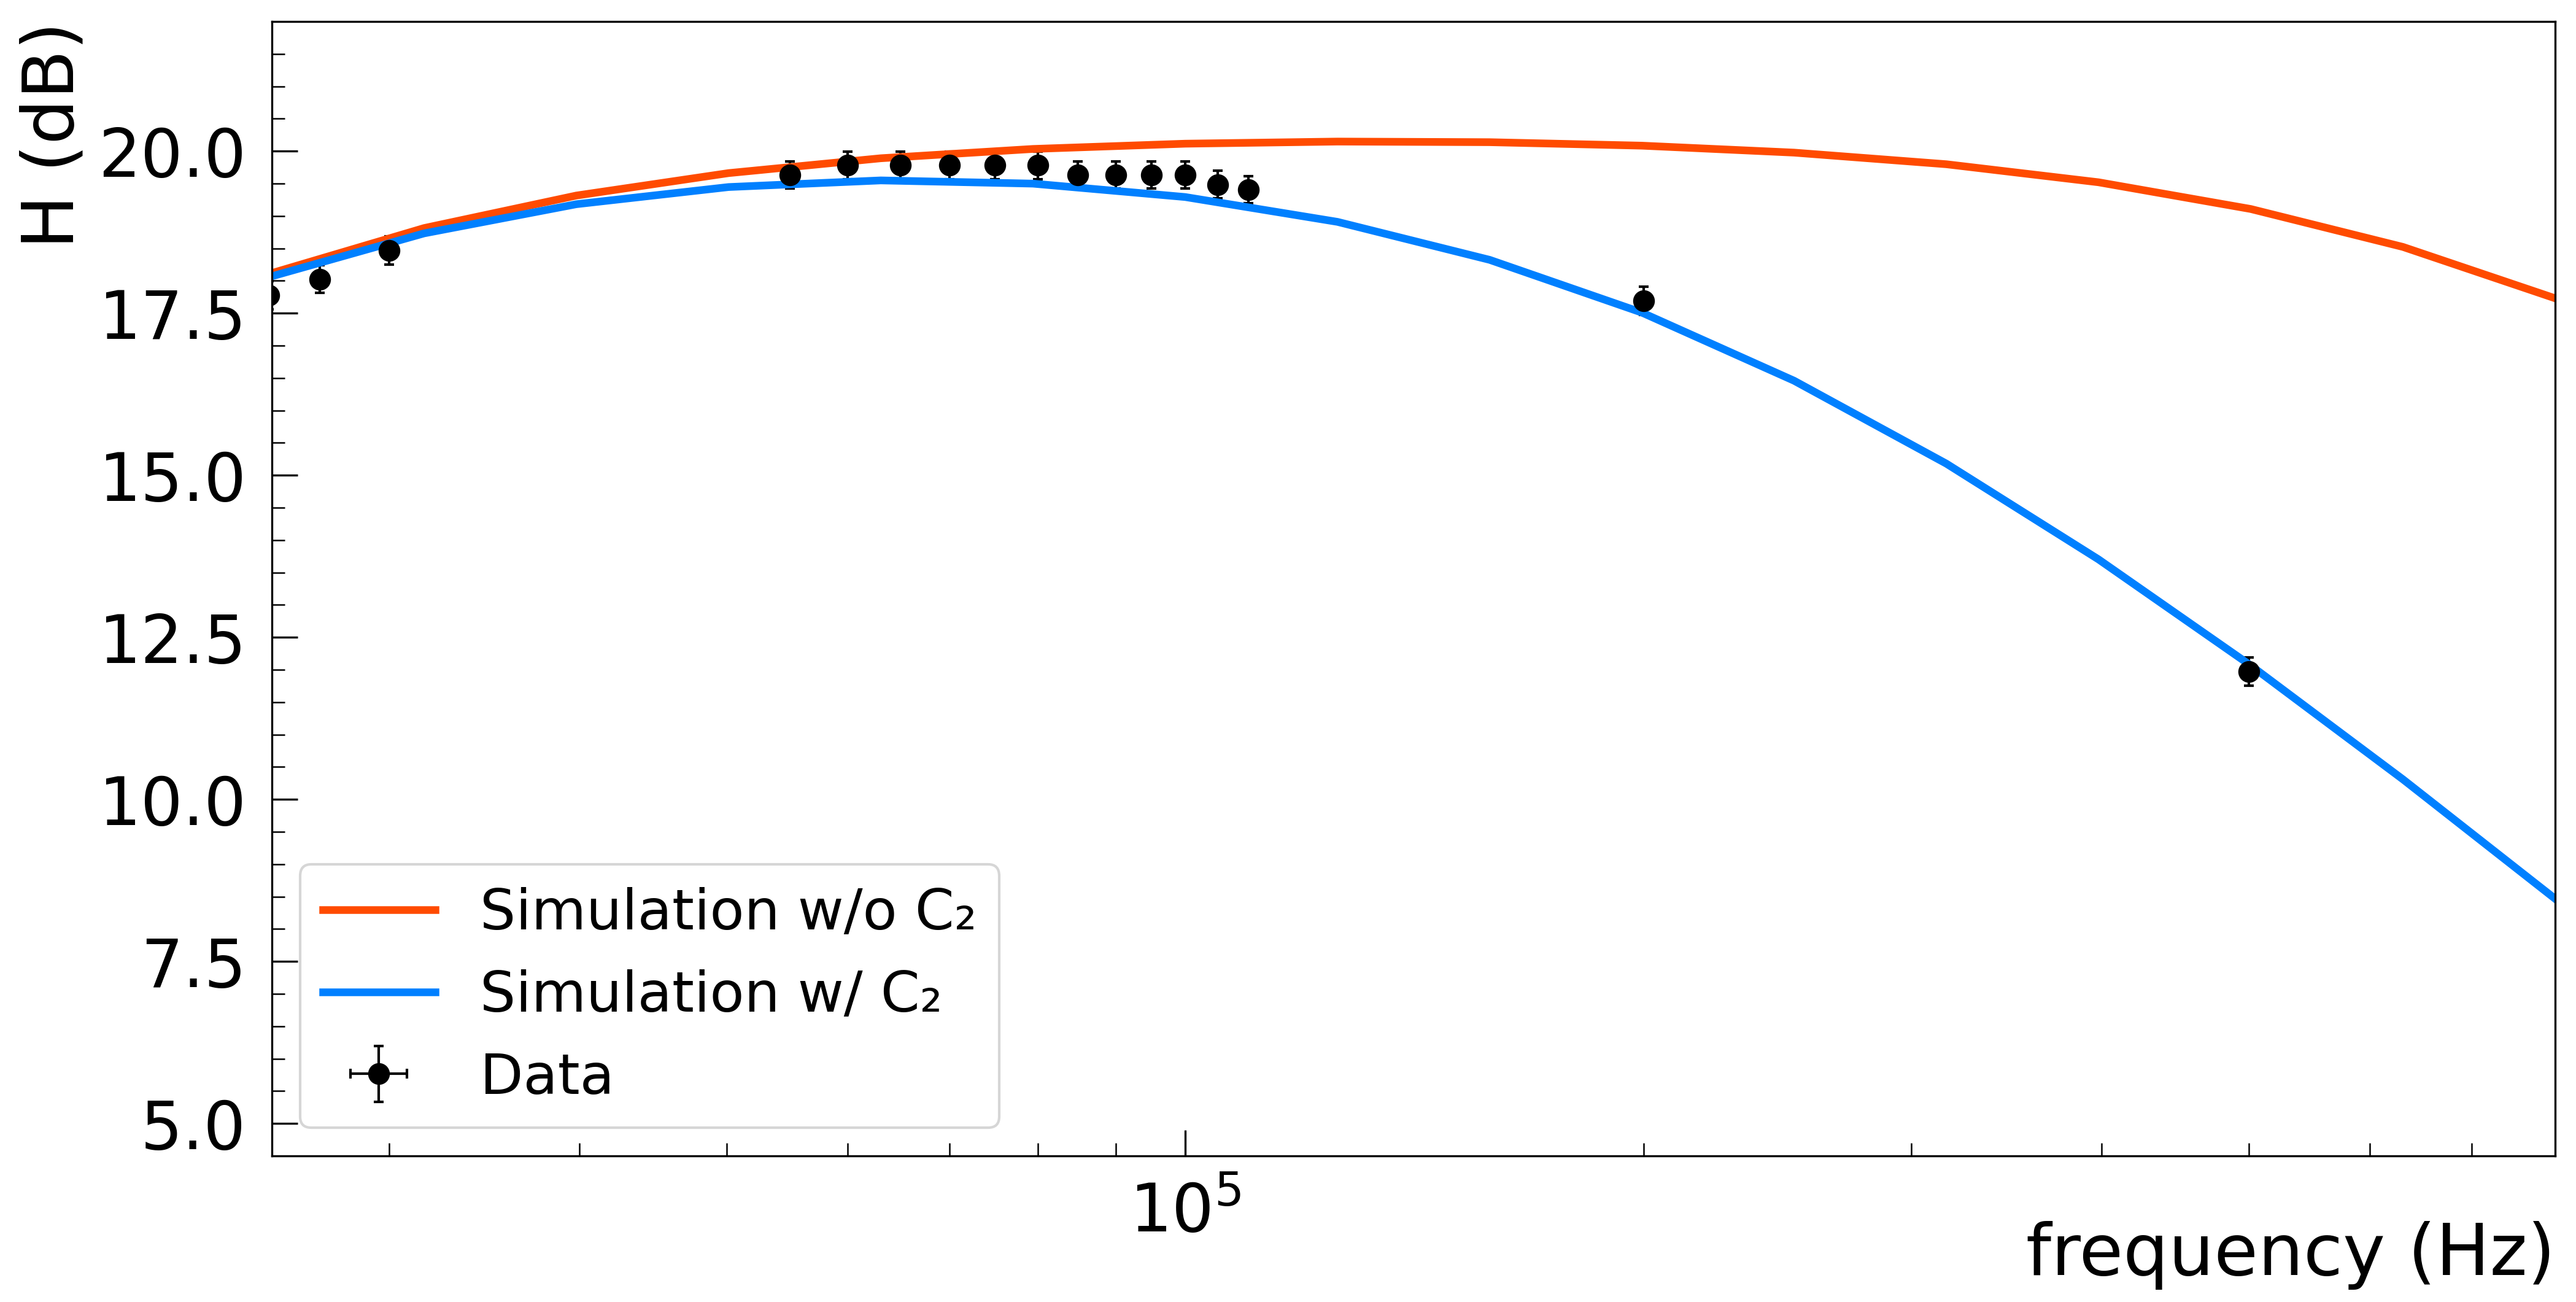
\includegraphics[width=0.5\textwidth]{../Plots/Report_Plots/diff_sim_comp.png}
	\caption{\small Confronto tra misure sperimentali e punti simulati con LTSpice.}
	\label{i:diff_sim_comp}
\end{wrapfigure}

\noindent Effettuando un'ulteriore simulazione, aggiungendo una capacità $C_{2}=7\,\si{\pF}$ in parallelo alla
resistenza di feedback $R_{\text{f}}$, si trova un notevole miglioramento nell'accordo tra punti simulati e misure
sperimentali: questo conferma dunque che l'effetto di attenuazione della funzione di trasferimento del circuito è dovuto
a dei contributi capacitivi non trascurabili posti in parallelo ad esso. In \autoref{i:diff_sim_comp} è messo in
evidenza questo confronto tra i dati sperimentali e quelli simulati, sia trascurando la capacità $C_{2}$ (in arancione)
sia invece tenendone conto (in azzurro). Si procede ora nella ricerca della frequenza di taglio del circuito. Si calcola
allora il massimo della funzione di trasferimento, facendo riferimento ai parametri del fit parabolico, come
$H_{\text{max}}=-\frac{d^2-4ce}{4c}=19.79\pm 0.05\,\text{dB}$, dove nel computo dell'errore sono state tenute in
considerazione le opportune covarianze tra i parametri. Successivamente, si calcola il punto di intersezione tra la
retta orizzontale passante per $H_{\text{max}}$ e la retta interpolante le prime misure secondo
$x_{\text{int}}=\frac{H_{\text{max}}-a}{b}=4.370 \pm 0.017\,\text{dec}$ (anche in questo caso nel computo dell'errore
sono state tenute in considerazione le opportune covarianze tra i parametri $a$ e $b$ della retta). Convertendo quanto
trovato in Hertz, la frequenza di taglio così stimata risulta essere $f_{\text{t}}=23.4 \pm 0.9\,\si{\Hz}$.\\
Tale valore è però incompatibile sia con le aspettative teoriche, sia con quanto trovato sperimentalmente, seppur in
modo approssimativo. Si vuole allora procedere stimando la frequenza di taglio utilizzando un metodo alternativo, con il
fine di verificare se questa incompatibilità con le aspettative risulta essere ricorrente. In particolare, si vuole
considerare sia la frequenza sia la funzione di trasferimento in scala lineare ed effettuare un fit del tipo $y = mx +
q$ in uno stretto intorno della frequenza di taglio. Ricordando poi che la frequenza di taglio è tale da attenuare la
funzione di trasferimento di un fattore $\sqrt{2}$, la prima può essere ricavata da
\begin{align}
	\frac{H_{\text{max}}}{\sqrt{2}}&=mx+q & \Longrightarrow & & f_{\text{t}}&=\frac{\frac{H_{\text{max}}}{\sqrt{2}}-q}{m}
\end{align}

\noindent Per effettuare il fit, il contributo di scala presente in \autoref{e:diff_err} non viene considerato in quanto
non altera l'andamento dei residui. Il contributo viene quindi aggiunto in secondo luogo sui parametri
dell’interpolazione, in particolare nel calcolo di $f_{\text{t}}$ come segue
\begin{equation}\label{e:diff_prop}
	\sigma_{f_{\text{t}}}=\sqrt{
		\left(
			\frac{\partial f_{\text{t}}}{\partial m}
			%\frac{q}{m^2}-\frac{H_{\text{max}}}{m^2\sqrt{2}}
		\right)^2\sigma_m^2+
		\left(
			\frac{\partial f_{\text{t}}}{\partial q}
			%-\frac{1}{m}
		\right)^2\sigma_q^2+
		%\left(
		%	\frac{\partial f_{\text{t}}}{\partial H}
		%\right)^2\sigma_{H}^2+
		2\left(
			\frac{H_{\text{max}}}{m\sqrt{2}}
		\right)^2\sigma_k^2+
		2\left(
			\frac{\partial f_{\text{t}}}{\partial m}
			%\frac{q}{m^2}-\frac{H_{\text{max}}}{m^2\sqrt{2}}
		\right)
		\left(
			\frac{\partial f_{\text{t}}}{\partial q}
			%-\frac{1}{m}
		\right)\text{cov}(m,q)
	}
\end{equation}

\noindent dove appunto $\sigma_{\text{k}}=1.5\%$ rappresenta il contributo di scala. Si sceglie allora come $H_{\text{max}} =
9.76 \pm 0.05$ il valore trovato attraverso il fit parabolico precedente (in scala lineare) e si estrapolano i parametri
$m$ e $q$ dal seguente fit nell'intervallo di frequenze 17 - 24 kHz. Si vuole far notare che in \autoref{e:diff_prop}
non è stato considerato il termine relativo ad $H_{\text{max}}$ per comodità, in quanto tale contributo si ritrova
essere due ordini di grandezza inferiore rispetto agli altri termini e non modifica in quantità apprezzabile la stima
finale dell'errore.

\begin{figure}[H]
	\centering
	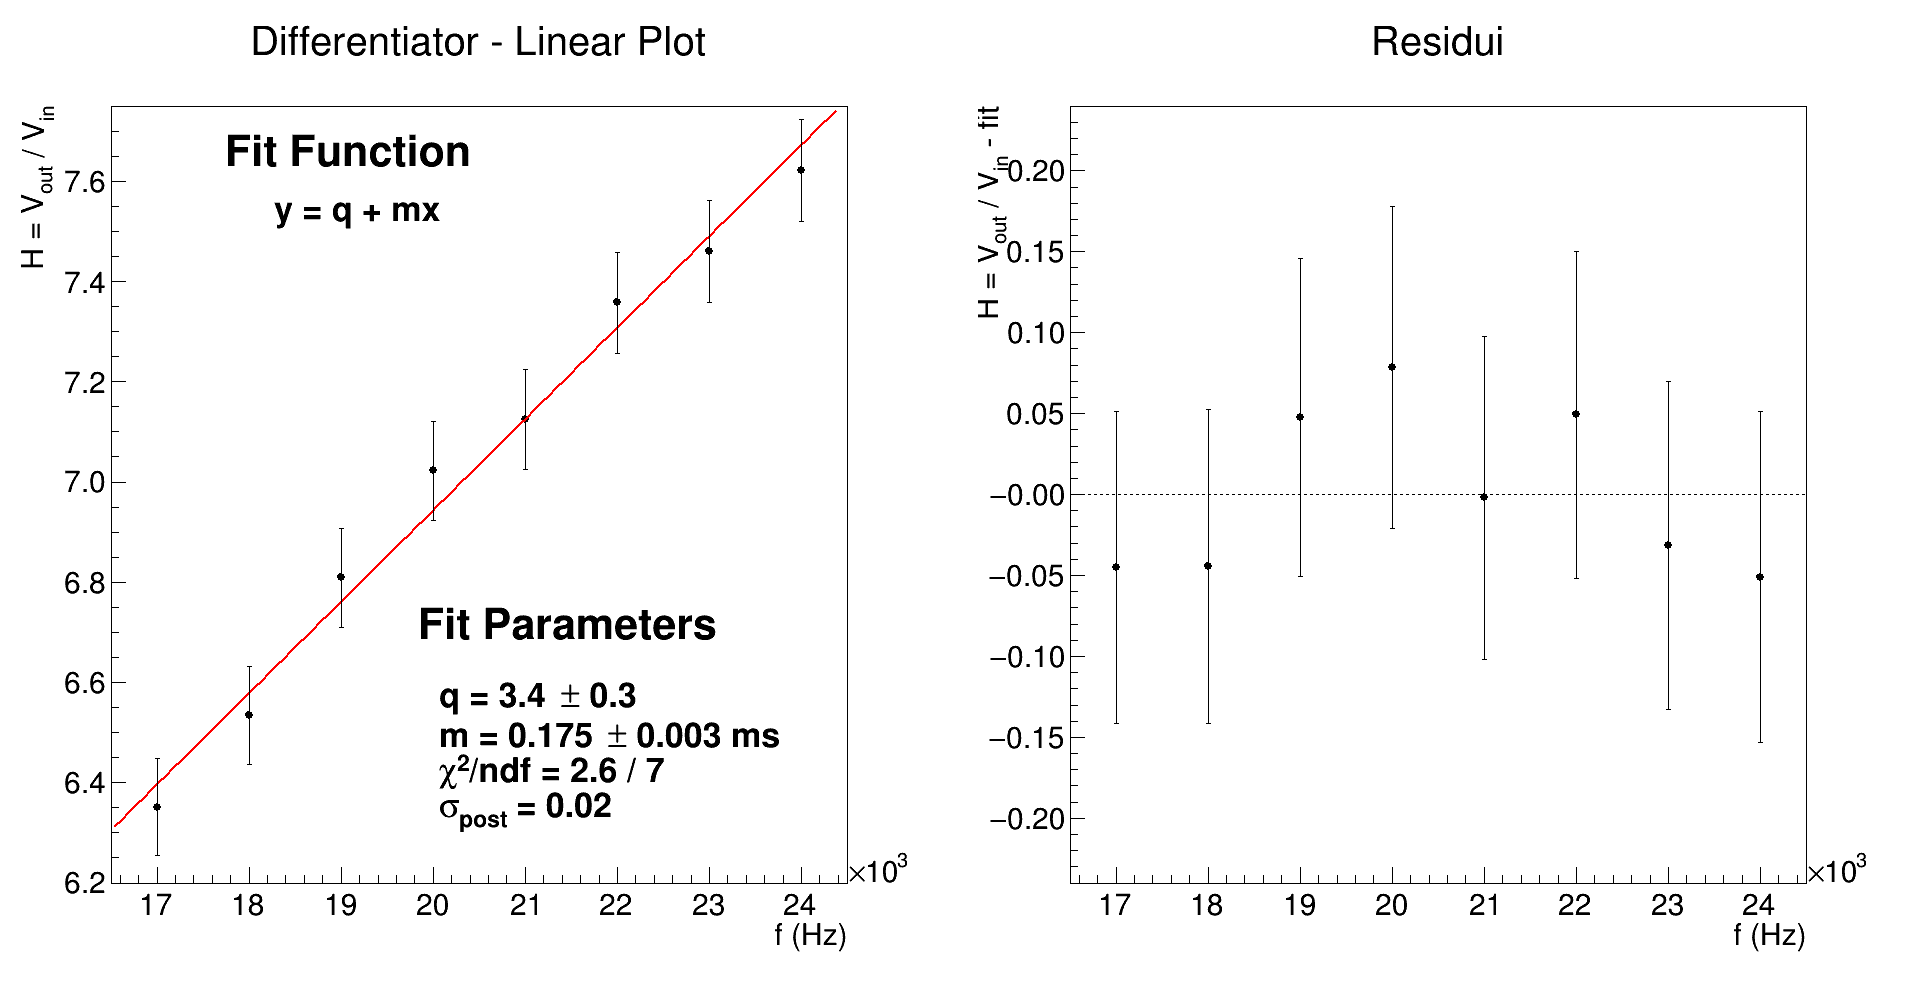
\includegraphics[width=\linewidth]{../Plots/Report_Plots/diff_linear.png}
	\caption{\small Interpolazione lineare delle misure in un intorno della frequenza di taglio e relativo grafico dei residui.}
	\label{i:diff_linear}
\end{figure}

\noindent Si nota immediatamente una leggera tendenza paraolica dell'andamento dei residui, tuttavia, pur avendo
trascurato il contributo di scala nel calcolo delle incertezze, i punti si distribuiscono tutti entro il loro errore. Il
$\chi^2$ risulta in ogni caso compatibile con il suo valore di aspettazione ($\lambda = 1.2$), pur segnalando una
possibile sovrastima dell'errore sulle misure (ipotesi assecondata anche dall'errore a posteriori, che risulta essere
circa $1/5$ rispetto alle incertezze assegnate ai dati). La stima della frequenza di taglio che si ottiene è dunque
$f_{\text{t}} = 19.8\pm 0.8\,\si{\kHz}$: questa risulta essere in ottimo accordo con le previsioni teoriche
($\lambda=0.4$) e, di conseguenza, si trova essere scarsamente compatibile con quanto ricavato studiando il grafico di
Bode ($\lambda = 3.0$).


%-------------------------------------------------------------------------------------------------------------------------------------------
%	ARDUINO
%-------------------------------------------------------------------------------------------------------------------------------------------

\section{Arduino}
In questa sezione si vuole effettuare una calibrazione della scheda Arduino Due. In particolare, si vuole quantificare
il sampling rate dell'ADC della scheda e determinare la funzione di calibrazione in tensione, ovvero $V = a + b \cdot
\text{ADC}$ dove $V$ è il valore in Volt del segnale, $\text{ADC}$ è la tensione in ADC counts acquisita da Arduino,
mentre $a$ e $b$ sono i parametri di calibrazione. Si ricorda che la scheda in questione presenta un ADC a 12 bit,
ovvero 4096 valori, e l'\textit{operating voltage} caratteristico (ovvero il valore massimo di tensione che può leggere
in input) è $V_{\text{op}}=3.3\,\si{\volt}$.\footnote{\url{https://www.arduino.cc/en/pmwiki.php?n=Main/arduinoBoardDue}}
La più piccola variazione di tensione rilevabile in ADC counts risulta dunque essere circa $0.8\,\si{\mV}$. Ci si
aspetta dunque di trovare una funzione di calibrazione in tensione con un coefficiente angolare attorno a tale valore. 

%-------------------------------------------------------------------------------------------------------------------------------------------
%	SAMPLING RATE 
%-------------------------------------------------------------------------------------------------------------------------------------------

\subsection{Sampling Rate}
Si comincia configurando il segnale di trigger. Si imposta quindi nel canale CH2 del generatore un impulso quadrato di
durata $10\,\si{\us}$, frequenza $1\,\si{k\hertz}$ e altezza $2\,\si{\volt}$ a partire dallo zero. Sul canale CH1 del
generatore, invece, si imposta un'onda quadra di ampiezza $1\,\si{\volt}$ partendo da zero con frequenza
$5\,\si{k\hertz}$. Conoscendo il periodo dell'onda quadra in ingresso ($T=1/f$), il sampling rate viene computato come
$S = N / T = N \, f$ con $N$ il numero di misure acquisite in un periodo. Per calcolare $N$ viene computata la derivata
numerica della forma d'onda: questa presenterà dei picchi positivi quando la funzione passa da zero a $1\,\si{\volt}$ e
picchi negativi quando scende da $1\,\si{\volt}$ a zero. Il numero di acquisizioni in un periodo sarà allora il numeri
di punti compresi tra due picchi positivi della funzione derivata. Si trova allora un sampling rate $S = 955000 s^{-1}$,
ovvero 955000 acquisizioni al secondo.


%-------------------------------------------------------------------------------------------------------------------------------------------
%	CALIBRAZIONE IN TENSIONE
%-------------------------------------------------------------------------------------------------------------------------------------------

\subsection{Calibrazione in Tensione}
Si vuole ora verificare la linearità dell'ADC interno alla scheda e stimare i parametri $a$, $b$ della funzione di
calibrazione, in quanto si è interessati a convertire il segnale acquisito da ADC counts in Volt. Si acquisiscono allora
diverse forme d'onda facendo variare la tensione del generatore, avendo cura di misurare il segnale erogato con i
cursori dell'oscilloscopio, in quanto può non essere esattamente uguale a quello nominale indicato dal generatore. Si
rappresentano in grafico i valori di tensione $V$ misurati sperimentalmente contro la media dei punti appartenenti ai
picchi della relativa forma d'onda (si decide di non considerare unicamente il massimo della forma in quanto è possibile
si tratti di una fluttuazione). Per quanto riguarda le incertezze associate ai dati, si associa lungo y l'errore
riportato in \autoref{e:osc} (misure acquisite utilizzando i cursori), mentre si assume che l'incertezza di acquisizione
delle misure di Arduino sia trascurabile rispetto a quella dell'oscilloscopio e non viene quindi considerata.
Effettuando poi un'interpolazione lineare, riportata in \autoref{i:ar_calib}, si ricavano l'offset (cioè quanti Volt
corrispondono allo zero dell'ADC) ed il coefficiente angolare (cioè come scalano i Volt rispetto all'ADC).
Osservando il grafico dei residui, si nota un marcato andamento anomalo dei punti a tensioni maggiori, oltre i
$2\,\si{\volt}$: la scheda, cioè, risponde in modo leggermente diverso a seconda della tensione in ingresso. Questo è,
molto probabilmente, dovuto al circuito di protezione dei pin di ingresso (limitatore di tensione a diodi, utile per
evitare di bruciare la scheda) che ne altera la risposta avvicinandosi a tensioni pericolose. Si prova allora ad
effettuare nuovamente l'interpolazione rimuovendo i punti relativi a tensioni in ingresso maggiori di $2\,\si{\volt}$:
nonostante l'andamento dei residui migliori, anche il primo punto (tensione in ingresso pari a $200\,\si{\mV}$) si trova
essere fuori trend. Si ottengono quindi due zone in cui la linearità dell'ADC risulta essere ottimale: la prima tra
$500\,\si{\mV}$ e $1.8\,\si{\volt}$ (parametri di calibrazione: $a = -0.59 \pm 0.02 \, \si{\V}$ e $b = 0.776 \pm 0.013
\,\si{\mV}/\text{a.u.}$) mentre la seconda tra $1.8\,\si{\volt}$ e $2.5\,\si{\volt}$ (parametri di calibrazione: $a =
-0.44 \pm 0.15 \, \si{\V}$ e $b = 0.73 \pm 0.04 \,\si{\mV}/\text{a.u.}$).

\begin{figure}[H]
	\centering
	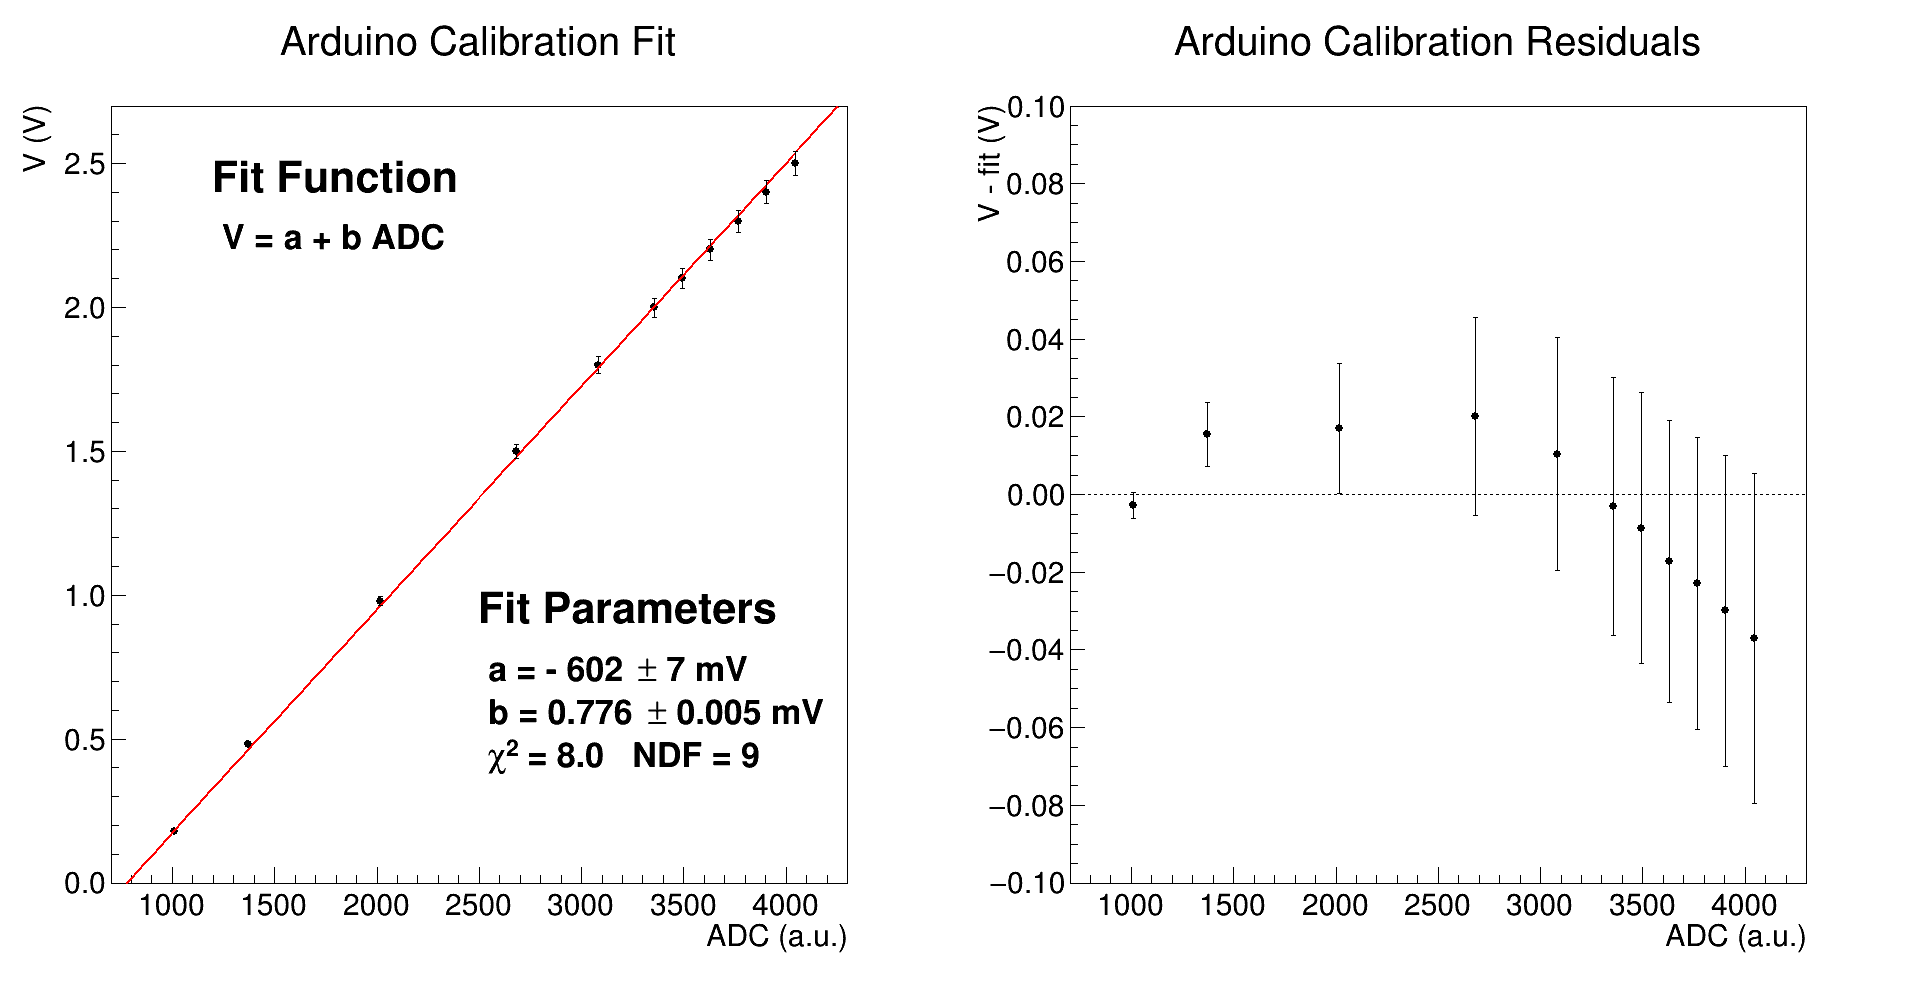
\includegraphics[width=15cm]{../Arduino/Plots/calib_function.png}
	\caption{Grafico di calibrazione in tensione e relativo grafico dei residui.}
	\label{i:ar_calib}
\end{figure}

\noindent 



%-------------------------------------------------------------------------------------------------------------------------------------------
%	CONCLUSIONI
%-------------------------------------------------------------------------------------------------------------------------------------------

\section{Conclusioni}
Ripercorrendo brevente quanto riscontrato nell'analisi effettuata, si vuole cominciare osservando che non è stato
possibile quantificare la linearità di un amplificatore operazionale studiando il $\chi^2$ restituito dalle
interpolazioni lineari, in quanto la correlazione tra errori di scala dell'oscilloscopio rendono i $\chi^2$ decisamente
ridotti rispetto al valore di aspettazione. L'andamento del grafico dei residui, in particolare ci si riferisce al fit
delle grandezze picco picco in \autoref{i:opamp_pp}, tuttavia conferma una soddisfacente linearità dell'operazionale.
Per quanto riguarda lo studio dell'amplificazione del circuito (rappresentato in \autoref{i:opamp_circuit}), sono stati
trovati risultati coonformi tra loro e con le aspettative teoriche considerando il campione di massimi ed il campione di
minimi separatamente. A causa di sistematiche di offset verticale tra i due campioni di misure il dataset unificato
(massimi e minimi) porta ad un'amplificazione, seppur leggermente compatibile, sensibilmente differente dalle
precedenti. L'amplificazione estrapolata considerando le grandezze picco picco, invece, risulta essere conforme sia con
le aspettative teoriche sia con le due stime ricavate considerando i campioni separati: siccome l'errore sulla stima
dell'amplificazione è, con buona probabilità, sottostimato, si sceglie come miglior stima di quest'ultima proprio quella
ottenuta considerando le grandezze picco picco $G=10.29 \pm 0.11$ in quanto presenta un errore leggermente maggiore
rispetto alla media pesata tra i valori di amplificazione ottenuti considerando il campione di massimi ed il campione di
minimi separatamente. Spostando ora l'attenzione verso il circuito derivatore, dall'analisi in frequenza è emerso un
comportamento più fedele ad un filtro passa banda piuttosto che un passa alto (cioè l'aspettativa teorica) e si è
ipotizzato che la causa fosse la presenza di una capacità parassita in parallelo al circuito. La frequenza di taglio
estrapolata attraverso la prima strategia si è ritrovata essere scarsamente compatibile con le aspettative teoriche, e
la causa di ciò potrebbe essere una campionatura troppo rarefatta a basse frequenze che ha portato ad una stima non
ottimale della retta a 20 dB/dec. L'interpolazione lineare ristretta all'intorno della frequenza di taglio, nel quale la
campionatura è sufficientemente fitta, invece restituisce una stima $f_{\text{t}}=19.8 \pm 0.8\,\si{\kHz}$ in ottimo
accordo con le aspettative. Si prende dunque quest'utlima come miglior stima della frequenza di taglio. Per quanto
riguarda la calibrazione della scheda Arduino Due, infine, si è stimato un sampling rate di 955000 acquisizioni al
secondo e una funzione di calibrazione conforme alle aspettative, ovvero con un coefficiente angolare $m=0.766\pm
0.013\,\text{mV/adc counts}$ e un offset $q=-0.59\pm0.02\,\si{\volt}$ per valori di tensione in ingresso sotto i circa
$2\,\si{\volt}$.



\end{document}